\documentclass[11pt,a4paper]{article}
\usepackage[T1]{fontenc}
\usepackage{lmodern}
\usepackage{microtype}
\usepackage[margin=2.4cm]{geometry}
\usepackage{graphicx}
\usepackage{booktabs}
\usepackage{tabularx}
\usepackage{array}
\usepackage{float}
\usepackage{caption}
\usepackage{subcaption}
\usepackage{xcolor}
\usepackage{enumitem}
\usepackage{titlesec}
\usepackage{fancyhdr}
\usepackage{amsmath}
\usepackage{siunitx}
\usepackage{tikz}
\usetikzlibrary{arrows.meta,positioning,shapes.geometric,fit,backgrounds}
\usepackage[hidelinks]{hyperref}

\graphicspath{{../../outputs/figures/}}
\sisetup{group-separator={,}, group-minimum-digits=4}
\captionsetup{font=small,labelfont=bf}
\setlist{itemsep=2pt,topsep=4pt}
\titleformat{\section}{\large\bfseries}{\thesection}{0.6em}{}
\titleformat{\subsection}{\normalsize\bfseries}{\thesubsection}{0.6em}{}
\definecolor{accent}{HTML}{1F5A96}
\pagestyle{fancy}
\fancyhf{}
\fancyhead[L]{\small Flood inundation and settlement exposure, Nagaon, June 2022}
\fancyhead[R]{\small\thepage}
\renewcommand{\headrulewidth}{0.4pt}
\newcommand{\kmsq}{km\textsuperscript{2}}
\setlength{\parskip}{4pt}
\setlength{\parindent}{0pt}

\begin{document}

% ------------------------------------------------------------------ title page
\begin{titlepage}
\centering
\vspace*{2.5cm}
{\color{accent}\rule{\linewidth}{1.2pt}}\\[0.6cm]
{\LARGE\bfseries Flood Inundation and Settlement Exposure\\[4pt] in Nagaon District, Assam, during June 2022}\\[0.4cm]
{\large Sentinel-1 SAR change detection with Google Earth Engine and Python}\\[0.4cm]
{\color{accent}\rule{\linewidth}{1.2pt}}\\[2cm]
{\large GIS Project Report}\\[1.5cm]
\begin{tabular}{ll}
Aadyant Neog & BT2024186\\
Jeswin Jose & BT2024142\\
\end{tabular}\\[2.5cm]
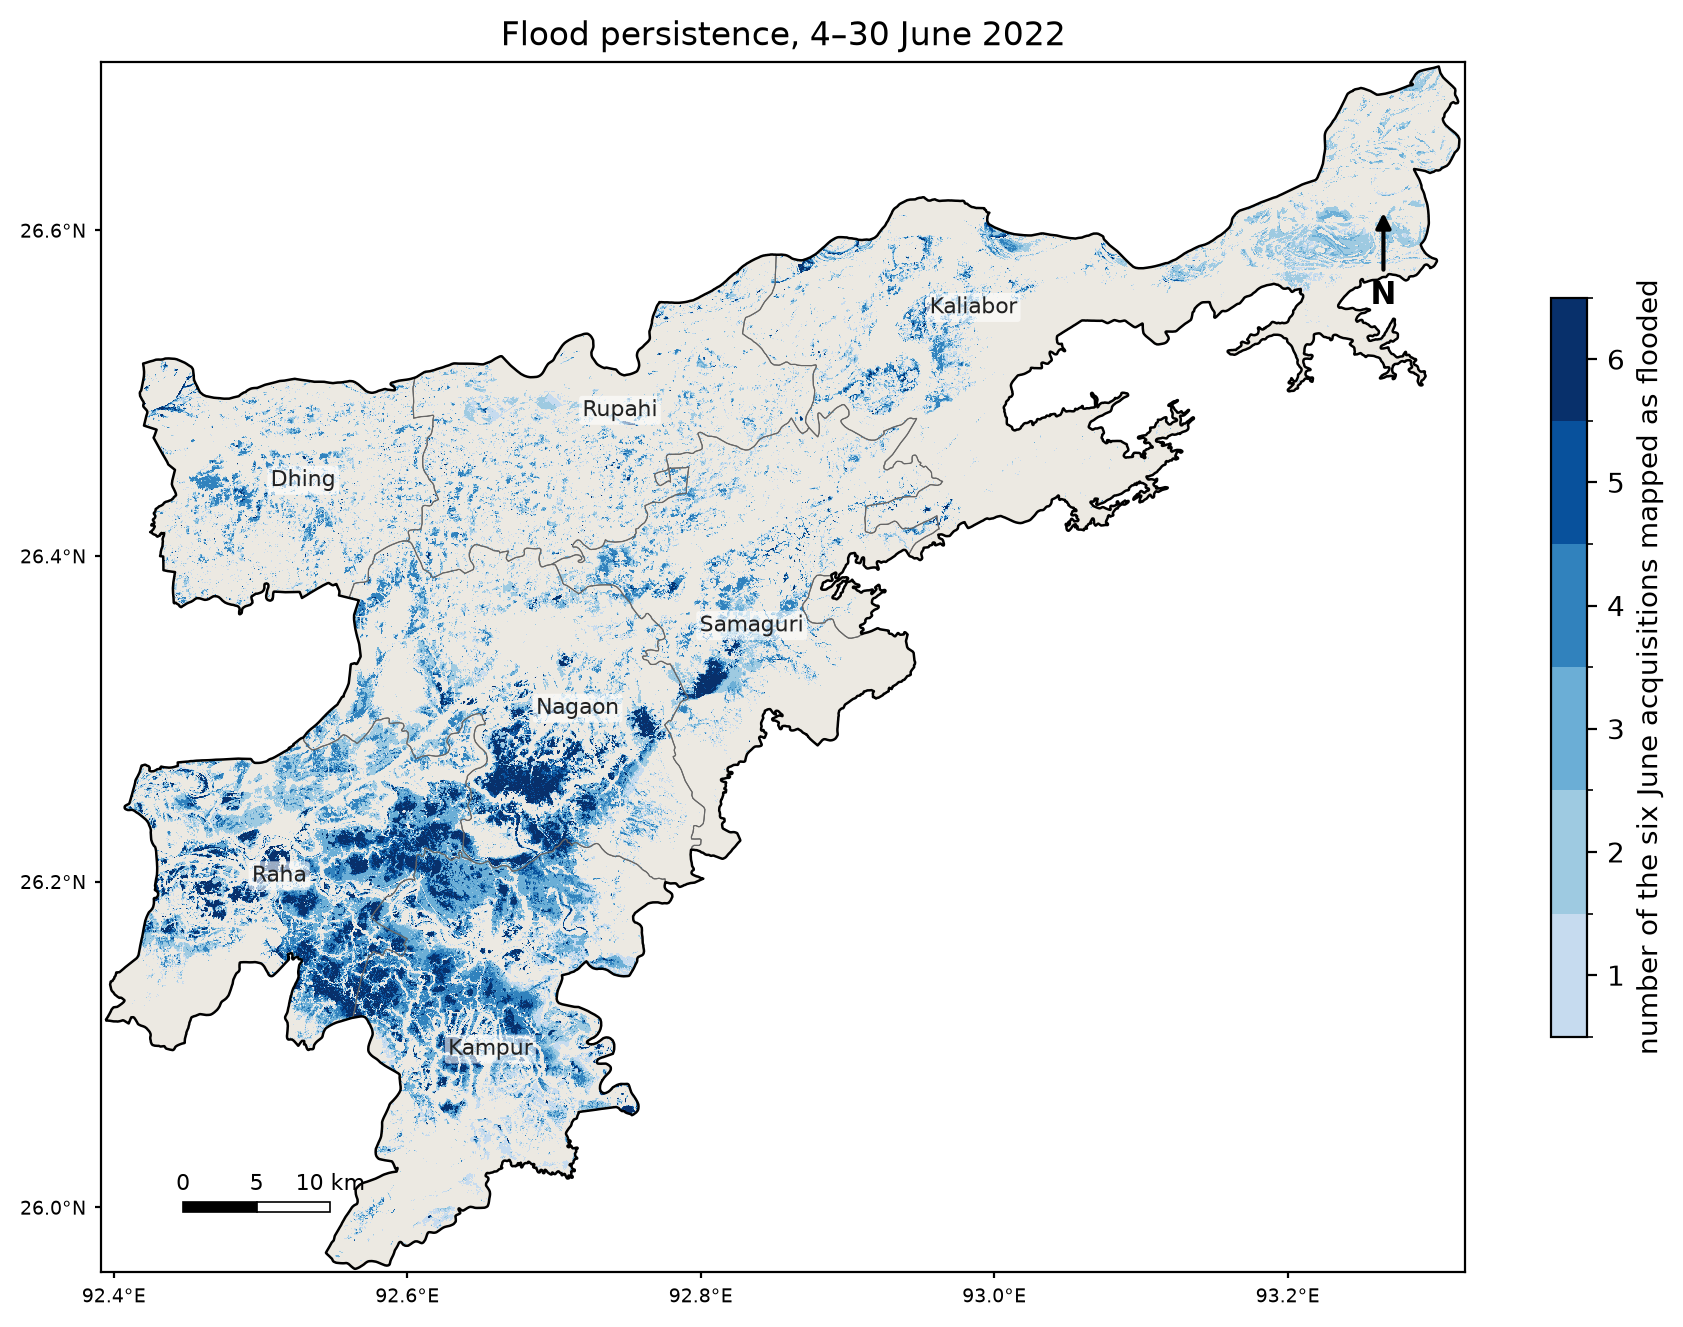
\includegraphics[width=0.62\linewidth]{map_flood_frequency.png}\\[1.2cm]
{\large November 2026}
\end{titlepage}

% ------------------------------------------------------------------ abstract
\section*{Abstract}
Monsoon floods in Assam recur every year, but cloud cover makes optical satellite images of
the flood peak scarce. This project mapped the June 2022 flood in Nagaon district with
Sentinel-1 synthetic aperture radar (SAR), which images the ground through cloud. Six
Sentinel-1A acquisitions from two orbit tracks (4, 6, 16, 18, 28 and 30 June) were compared with
same-track dry-season baselines using VH backscatter change detection with an automatic,
edge-based Otsu threshold. Terrain (height above nearest drainage, slope), permanent water and
small patches were excluded. Mapped flooding rose from \SIrange{124}{143}{\kmsq} in early June to
\SI{503}{\kmsq} on 18 June and \SI{600}{\kmsq} on 30 June; \SI{766}{\kmsq} (30\% of the district) was
flooded on at least one date. Because SAR cannot detect water among buildings, settlement exposure
was measured as ESA WorldCover built-up land within a distance of flood water: \SI{7.2}{\kmsq}
(11\% of the district's built-up area) lay within \SI{50}{m} of flooding on some June date, with the
highest shares in Raha (25\%) and Kampur (23\%). The flooded area was most sensitive to the
backscatter-drop threshold (\SIrange{423}{575}{\kmsq} on 18 June over common threshold choices) and
insensitive to terrain masks. The 30 June area agrees with the NRSC figure within 1\%; pixel
agreement with independent rapid-mapping products is moderate, and the comparison with an
L-band ALOS-2 map shows that flooding under tree canopy is missed by C-band Sentinel-1.

\noindent\textbf{Keywords:} flood inundation; Sentinel-1 SAR; change detection; settlement exposure; Nagaon; GIS

\newpage
\tableofcontents
\newpage

% ------------------------------------------------------------------ 1
\section{Introduction}
\subsection{Background}
Assam lies in the Brahmaputra valley and is flooded almost every monsoon. In 2022 the state was hit
by two major waves: in mid-May and again in the second half of June, when heavy rain and rising
water levels in the Brahmaputra and its tributaries inundated large parts of the valley. Nagaon district,
on the south bank of the Brahmaputra and drained by the Kopili and Kolong rivers, was among the
worst-affected districts in both waves.

Flood mapping during the monsoon is hampered by persistent cloud, which limits optical sensors.
Synthetic aperture radar is an active microwave sensor that images through cloud and at night.
Calm open water reflects the radar pulse away from the sensor (specular reflection) and appears dark,
so a sharp drop in backscatter between a dry reference image and an image acquired during the
flood indicates new inundation. The Copernicus Sentinel-1 mission acquires C-band SAR data
systematically over India and the data are freely available, which makes it suitable for district-scale
flood mapping \cite{twele}. A recent study of the same district and dates compared several
classifiers on Sentinel-1 data \cite{irukumati}.

\subsection{Problem statement}
This project delineates event-related inundation in Nagaon during June 2022, distinguishes it from
existing water bodies, and estimates its proximity to mapped built-up land in order to assess settlement
exposure at district scale.

\subsection{Objectives}
\begin{enumerate}
\item Map inundation on the available June 2022 Sentinel-1 observation dates.
\item Quantify flooded area and exposed built-up area.
\item Assess agreement with reference flood maps and sensitivity to detection thresholds.
\end{enumerate}

\subsection{Research questions}
\begin{enumerate}[label=(\roman*)]
\item How did observed inundation vary between June acquisition dates?
\item Where did inundation overlap (or lie close to) mapped built-up land?
\item How sensitive are flood extent and exposure estimates to the detection thresholds?
\end{enumerate}

% ------------------------------------------------------------------ 2
\section{Study area}
Nagaon district lies between about \ang{92.4}--\ang{93.3}\,E and \ang{25.96}--\ang{26.70}\,N in central
Assam (Figure~\ref{fig:study}). The boundary used corresponds to the district as constituted in June 2022:
Hojai, carved out of Nagaon in 2016, was still separate (it was re-merged only on 31 December 2022). The
boundary encloses \SI{2577.6}{\kmsq} (geodesic area) and matches the study area of \cite{irukumati}; a
second source (geoBoundaries, 2021) gives \SI{2508}{\kmsq} and was used as a cross-check. Seven
2011-census sub-districts fall inside the 2022 district and are used as reporting units: Kaliabor, Samaguri,
Rupahi, Dhing, Nagaon, Raha and Kampur. Most of the district is flat floodplain: 95\% of it lies less than
\SI{15}{m} above the nearest drainage line, and higher ground is limited to the hills along the southern
and eastern edges. Land cover (ESA WorldCover 2021) is dominated by cropland (51\%) and tree cover,
including village homestead gardens (39\%); built-up land covers \SI{63.9}{\kmsq} (2.5\%).

\begin{figure}[H]
\centering
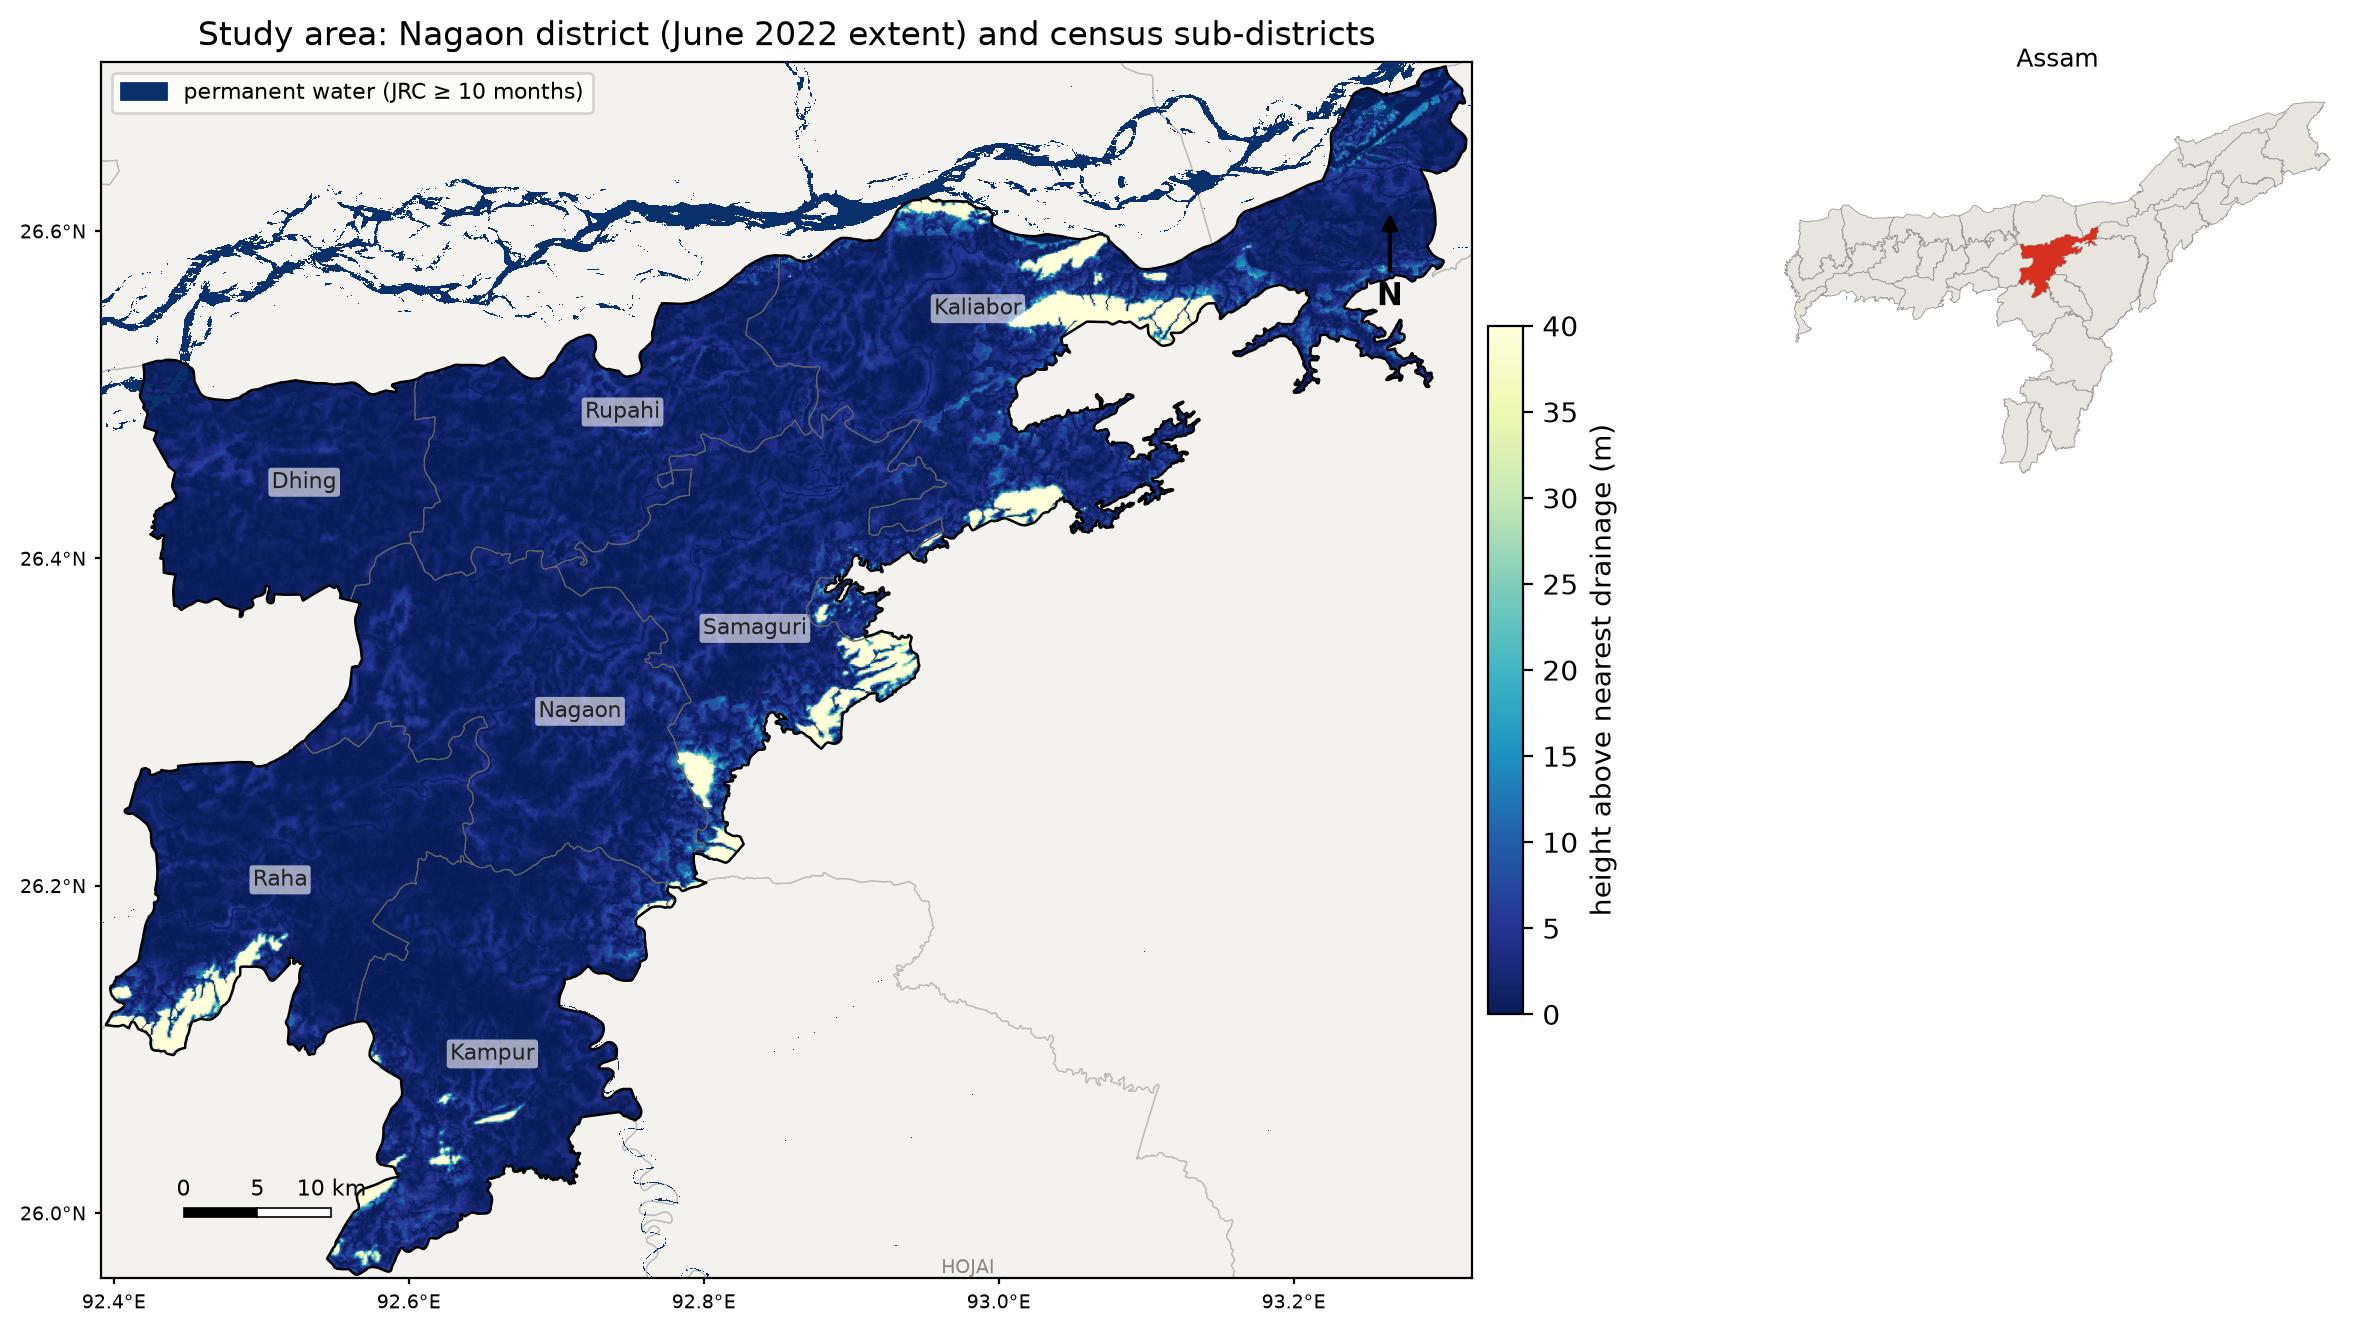
\includegraphics[width=\linewidth]{map_study_area.png}
\caption{Study area: Nagaon district (June 2022 extent) and census sub-districts, shaded by height above
nearest drainage (MERIT Hydro). Permanent water (JRC, $\geq$10 months per year) is shown in dark blue;
the Brahmaputra lies along the northern boundary.}
\label{fig:study}
\end{figure}

% ------------------------------------------------------------------ 3
\section{Data}
\begin{table}[H]
\centering\small
\caption{Datasets used.}
\label{tab:data}
\begin{tabularx}{\linewidth}{>{\raggedright}p{4.6cm}>{\raggedright}p{3.0cm}X}
\toprule
Dataset & Resolution & Use\\
\midrule
Sentinel-1A IW GRD (VV, VH), via Google Earth Engine & \SI{10}{m} & flood detection (6 event dates, 17 baseline scenes)\\
MERIT Hydro: HAND and DEM & \SI{90}{m} & terrain exclusions (HAND, slope)\\
JRC Global Surface Water v1.4 (1984--2021) & \SI{30}{m} & permanent and historical water\\
ESA WorldCover 2021 v200 & \SI{10}{m} & built-up land (class 50), land cover\\
District and sub-district boundaries (datta07/INDIAN-SHAPEFILES; geoBoundaries 2021) & vector & study area, reporting units\\
MBRSC flood map, Sentinel-1, 16 June 2022 (Sentinel Asia) & vector & reference (same scene as ours)\\
EOS-RS Flood Proxy Map, ALOS-2 PALSAR-2 (L-band), 22 June 2022 (Sentinel Asia) & vector & independent reference\\
EOS-RS Flood Proxy Map, Sentinel-1, 18 May 2022 (Sentinel Asia) & vector & May flood wave, baseline check\\
NRSC reference areas and classifier results \cite{irukumati} & table & published estimates\\
\bottomrule
\end{tabularx}
\end{table}

\paragraph{Sentinel-1 acquisitions.} Sentinel-1B failed in December 2021, so in 2022 each orbit track
was revisited only every 12 days. An inventory of all IW scenes over the district from January to July
2022 found three tracks. Two were used (Table~\ref{tab:s1}); the third (ascending track 143) covers only
55\% of the district. Scene dates are in UTC: the descending passes occur at 23:47~UTC, i.e.\ 05:17~IST
on the following morning, and the ascending passes at about 18:00~IST on the same day.

\begin{table}[H]
\centering\small
\caption{Sentinel-1A tracks and dates used.}
\label{tab:s1}
\begin{tabular}{lllcc}
\toprule
Track & Pass & June 2022 event dates (UTC) & District coverage & Baseline scenes\\
\midrule
77 & Descending & 6, 18, 30 June & 100\% & 8\\
41 & Ascending & 4, 16, 28 June & 93\% & 9\\
\bottomrule
\end{tabular}
\end{table}

\paragraph{Choice of baseline.} Nagaon was flooded during the mid-May 2022 wave
(the EOS-RS map of 18 May shows \SI{94.6}{\kmsq} of flooding inside the district). A May reference image,
as used in some earlier work, could therefore already contain flood water. The baseline was instead built
from the January to mid-April scenes of the same track.

% ------------------------------------------------------------------ 4
\section{Methodology}
The workflow (Figure~\ref{fig:flow}) splits the work between Google Earth Engine (GEE), used for data
access and per-scene preprocessing, and Python, used for classification, statistics and the sensitivity
analysis. All layers were placed on one \SI{10}{m} grid in UTM zone 46N (EPSG:32646), so areas are
computed in an equal-distance metric projection. QGIS-ready GeoTIFFs and styles were produced for
cartography.

\begin{figure}[H]
\centering
\resizebox{\linewidth}{!}{%
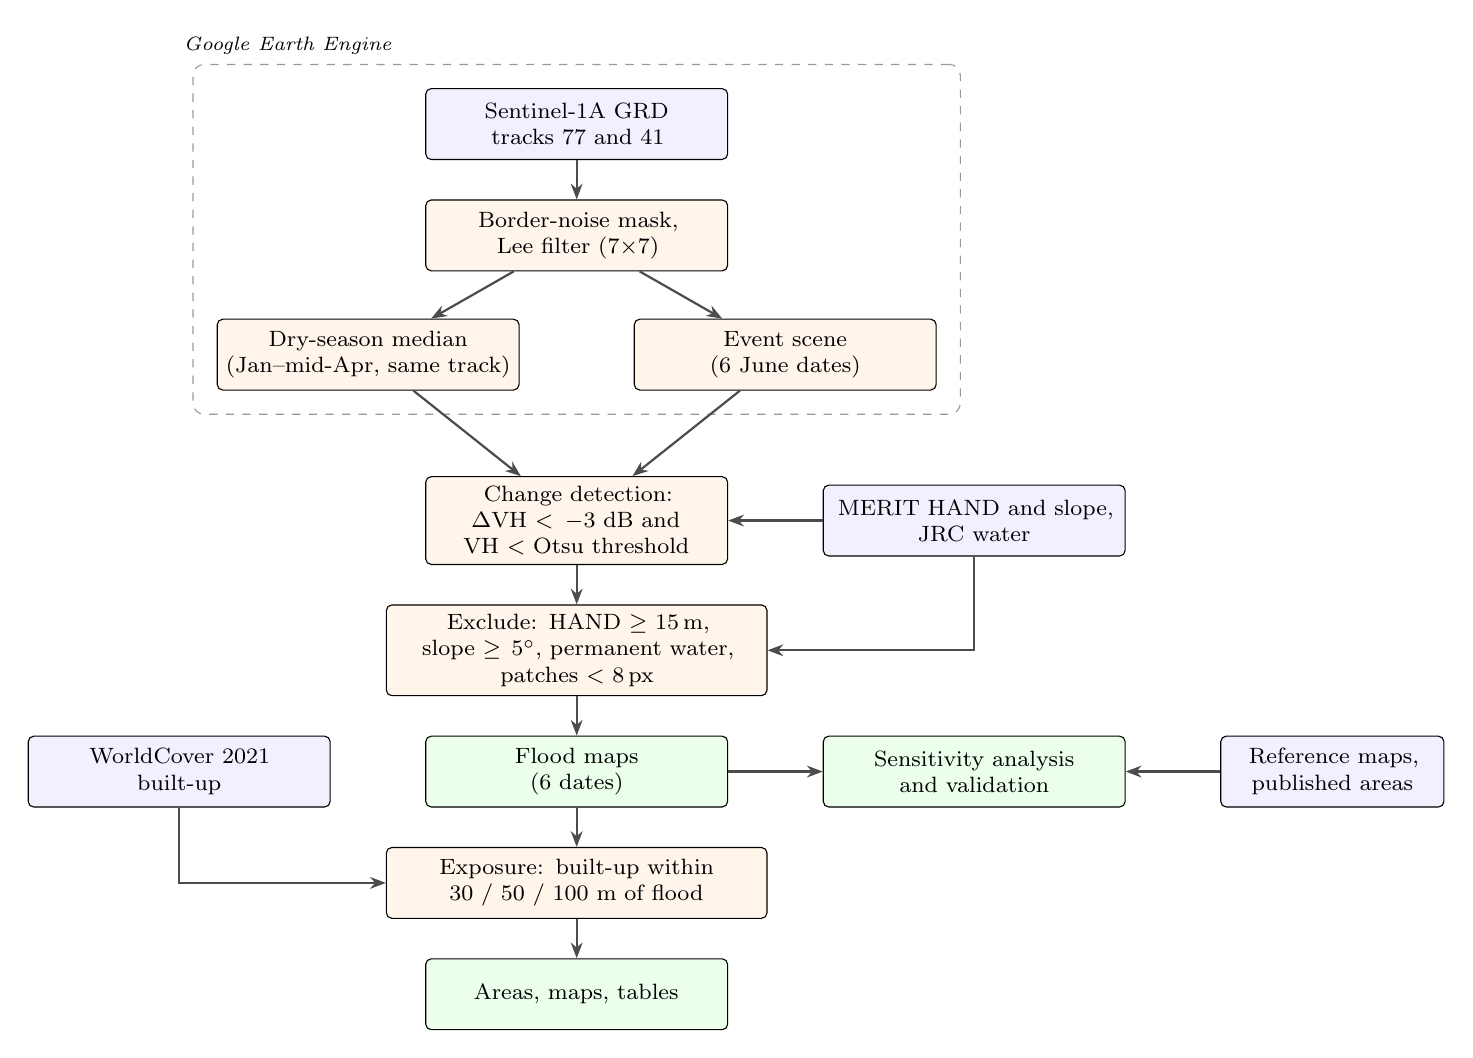
\begin{tikzpicture}[
  node distance=5mm and 8mm,
  box/.style={draw, rounded corners=2pt, align=center, font=\footnotesize, minimum height=9mm, text width=3.6cm, fill=white},
  data/.style={box, fill=blue!6},
  proc/.style={box, fill=orange!8},
  result/.style={box, fill=green!8},
  arr/.style={-{Stealth[length=2mm]}, thick, draw=black!70}]
\node[data] (s1) {Sentinel-1A GRD\\tracks 77 and 41};
\node[proc, below=of s1] (pre) {Border-noise mask,\\Lee filter (7$\times$7)};
\node[proc, below left=6mm and -1.2cm of pre] (base) {Dry-season median\\(Jan--mid-Apr, same track)};
\node[proc, below right=6mm and -1.2cm of pre] (ev) {Event scene\\(6 June dates)};
\node[proc, below=26mm of pre] (cd) {Change detection:\\$\Delta$VH $< -3$ dB and\\VH $<$ Otsu threshold};
\node[data, right=12mm of cd] (aux) {MERIT HAND and slope,\\JRC water};
\node[proc, below=of cd, text width=4.6cm] (ex) {Exclude: HAND $\geq$ 15\,m,\\slope $\geq 5^\circ$, permanent water,\\patches $<$ 8\,px};
\node[result, below=of ex] (fm) {Flood maps\\(6 dates)};
\node[data, left=12mm of fm] (wc) {WorldCover 2021\\built-up};
\node[proc, below=of fm, text width=4.6cm] (expo) {Exposure: built-up within\\30 / 50 / 100 m of flood};
\node[result, right=12mm of fm] (val) {Sensitivity analysis\\and validation};
\node[data, right=12mm of val, text width=2.6cm] (ref) {Reference maps,\\published areas};
\node[result, below=of expo] (res) {Areas, maps, tables};
\begin{scope}[on background layer]
\node[draw=black!40, dashed, rounded corners, fit=(s1)(pre)(base)(ev), inner sep=3mm, label={[font=\scriptsize\itshape]above left:Google Earth Engine}] {};
\end{scope}
\draw[arr] (s1) -- (pre);
\draw[arr] (pre) -- (base); \draw[arr] (pre) -- (ev);
\draw[arr] (base) -- (cd); \draw[arr] (ev) -- (cd);
\draw[arr] (aux) -- (cd); \draw[arr] (aux) |- (ex);
\draw[arr] (cd) -- (ex); \draw[arr] (ex) -- (fm);
\draw[arr] (fm) -- (expo); \draw[arr] (wc) |- (expo);
\draw[arr] (fm) -- (val); \draw[arr] (ref) -- (val);
\draw[arr] (expo) -- (res);
\end{tikzpicture}}
\caption{Processing workflow.}
\label{fig:flow}
\end{figure}

\subsection{Preprocessing}
The GEE Sentinel-1 GRD collection is already calibrated to $\sigma^0$ (dB), thermal-noise corrected and
terrain corrected with the SRTM DEM. For each scene, low-value border noise was masked
(VV $< -30$ dB) and speckle was reduced with a Lee filter \cite{lee} on linear intensity
(7$\times$7 window, equivalent number of looks 4.4). The dry-season baseline for each track is the
pixel-wise median of its filtered January to mid-April scenes. The VV and VH bands of each event
scene and of its baseline were exported as one stack per date.

\subsection{Flood classification}
A pixel was classed as flooded when both conditions held:
\begin{equation}
\mathrm{VH}_{\text{event}} - \mathrm{VH}_{\text{baseline}} < \Delta_{\text{VH}} = -3\ \text{dB}
\quad\text{and}\quad
\mathrm{VH}_{\text{event}} < T_{\text{VH}} .
\end{equation}
The first condition requires a significant darkening relative to dry conditions; the second requires the
pixel to look like open water on the event date. $T_{\text{VH}}$ was found automatically for each scene
with Otsu's method applied only to pixels within about \SI{60}{m} of land--water edges (detected with a
Canny filter) in flood-prone terrain, so that the histogram contains comparable numbers of water and land
pixels \cite{donchyts}. This plays the same role as the tile-based automatic thresholding in
\cite{twele}. The derived thresholds ranged from $-19.1$ to $-20.7$ dB, inside the usual range for open
water in VH, so the fixed fallback of $-20$ dB was never needed.

Following \cite{twele}, likely false positives were then removed:
\begin{itemize}
\item \textbf{HAND $\geq$ \SI{15}{m}}: terrain too high above the drainage network to flood.
\item \textbf{Slope $\geq \ang{5}$}, from the MERIT DEM. SRTM-derived slope was tested first but rejected: tree and
building heights make the SRTM surface rough, and more than 10\% of the lowest-lying land (HAND $<$ \SI{5}{m})
had SRTM slopes above \ang{5}, so the mask would have removed 12.7\% of flood-prone land. With the MERIT DEM,
which has vegetation bias removed, this fell to 1.1\%.
\item \textbf{Permanent water}: JRC seasonality $\geq$ 10 months per year (classed separately).
\item \textbf{Minimum mapping unit}: connected flood patches smaller than 8 pixels (\SI{800}{m^2}).
\end{itemize}
Each map has the classes \emph{not flooded}, \emph{flood}, \emph{permanent water} and \emph{not observed}.
Because track 41 misses the eastern tip of the district, areas are also reported for the footprint observed on all
six dates.

\subsection{Settlement exposure}
Built-up land was taken from WorldCover 2021 (class 50). A direct intersection of the flood maps with
built-up pixels is almost empty (\SI{0.14}{\kmsq} over all dates combined): buildings act as corner
reflectors (double bounce) and remain bright even when surrounded by water, so SAR flood maps cannot
show water among buildings. Exposure was therefore defined as built-up land within a given Euclidean
distance of mapped flood water, using \SI{50}{m} as the main distance and \SI{30}{m} and \SI{100}{m} as
alternatives. Results are reported per date, for the union of all dates, per sub-district, for 8-connected
built-up clusters, and on a \SI{1}{km} grid. Exposure indicates spatial proximity to inundation, not
confirmed damage or affected population.

\subsection{Sensitivity analysis and validation}
Each parameter was varied in turn around the default (the Otsu value held fixed) on three dates:
16 June (track 41), 18 June and 30 June (track 77). Parameters: VH-drop threshold ($-1$ to $-6$ dB),
absolute VH threshold ($-17$ to $-24$ dB), HAND (5--30 m and off), slope (\ang{2}--\ang{10} and off),
permanent-water definition (JRC $\geq$1 to 12 months, or none), minimum patch (1--100 px) and polarisation
(VH vs VV). A joint grid of the two main thresholds was also run for 18 June.

The maps were compared with the MBRSC map from the same 16 June scene and with the EOS-RS ALOS-2 map of
22 June, which uses an independent L-band sensor and lies between our 18 and 28 June scenes. Precision,
recall, F1, overall accuracy and Cohen's $\kappa$ were computed on all observed pixels, flood fractions were
compared at 100\,m, 500\,m and 1\,km, and disagreements were broken down by land cover. Total areas were
compared with the NRSC figures and classifier results reported by \cite{irukumati}.

% ------------------------------------------------------------------ 5
\section{Results}
\subsection{Flood extent through June (RQ i)}
Table~\ref{tab:area} and Figures~\ref{fig:six}--\ref{fig:ts} show how the flood developed. Flooding was limited in
early June (about 5\% of the district), increased sharply between 6 and 18 June, and was still at or near its
maximum at the end of the month. Both tracks show the same trajectory in the common footprint, which indicates
that the increase is not an artefact of viewing geometry. The automatic thresholds were very stable
($-19.1$ to $-20.7$ dB).

\begin{table}[H]
\centering\small
\caption{Flooded area by acquisition date.}
\label{tab:area}
\begin{tabular}{llrrrr}
\toprule
Date (UTC) & Track & Observed (\kmsq) & Flooded (\kmsq) & Common footprint$^{a}$ (\kmsq) & $T_{\text{VH}}$ (dB)\\
\midrule
4 June & 41 asc. & 2397.5 & 142.8 & 139.8 & $-20.0$\\
6 June & 77 desc. & 2574.8 & 124.4 & 116.0 & $-19.1$\\
16 June & 41 asc. & 2398.0 & 303.1 & 298.6 & $-19.9$\\
18 June & 77 desc. & 2574.0 & 503.4 & 468.4 & $-20.0$\\
28 June & 41 asc. & 2395.2 & 559.0 & 555.5 & $-20.7$\\
30 June & 77 desc. & 2573.2 & 600.1 & 560.4 & $-19.9$\\
\bottomrule
\end{tabular}\\[2pt]
{\footnotesize $^{a}$ flooded area inside the footprint observed on all six dates.}
\end{table}

\begin{figure}[H]
\centering
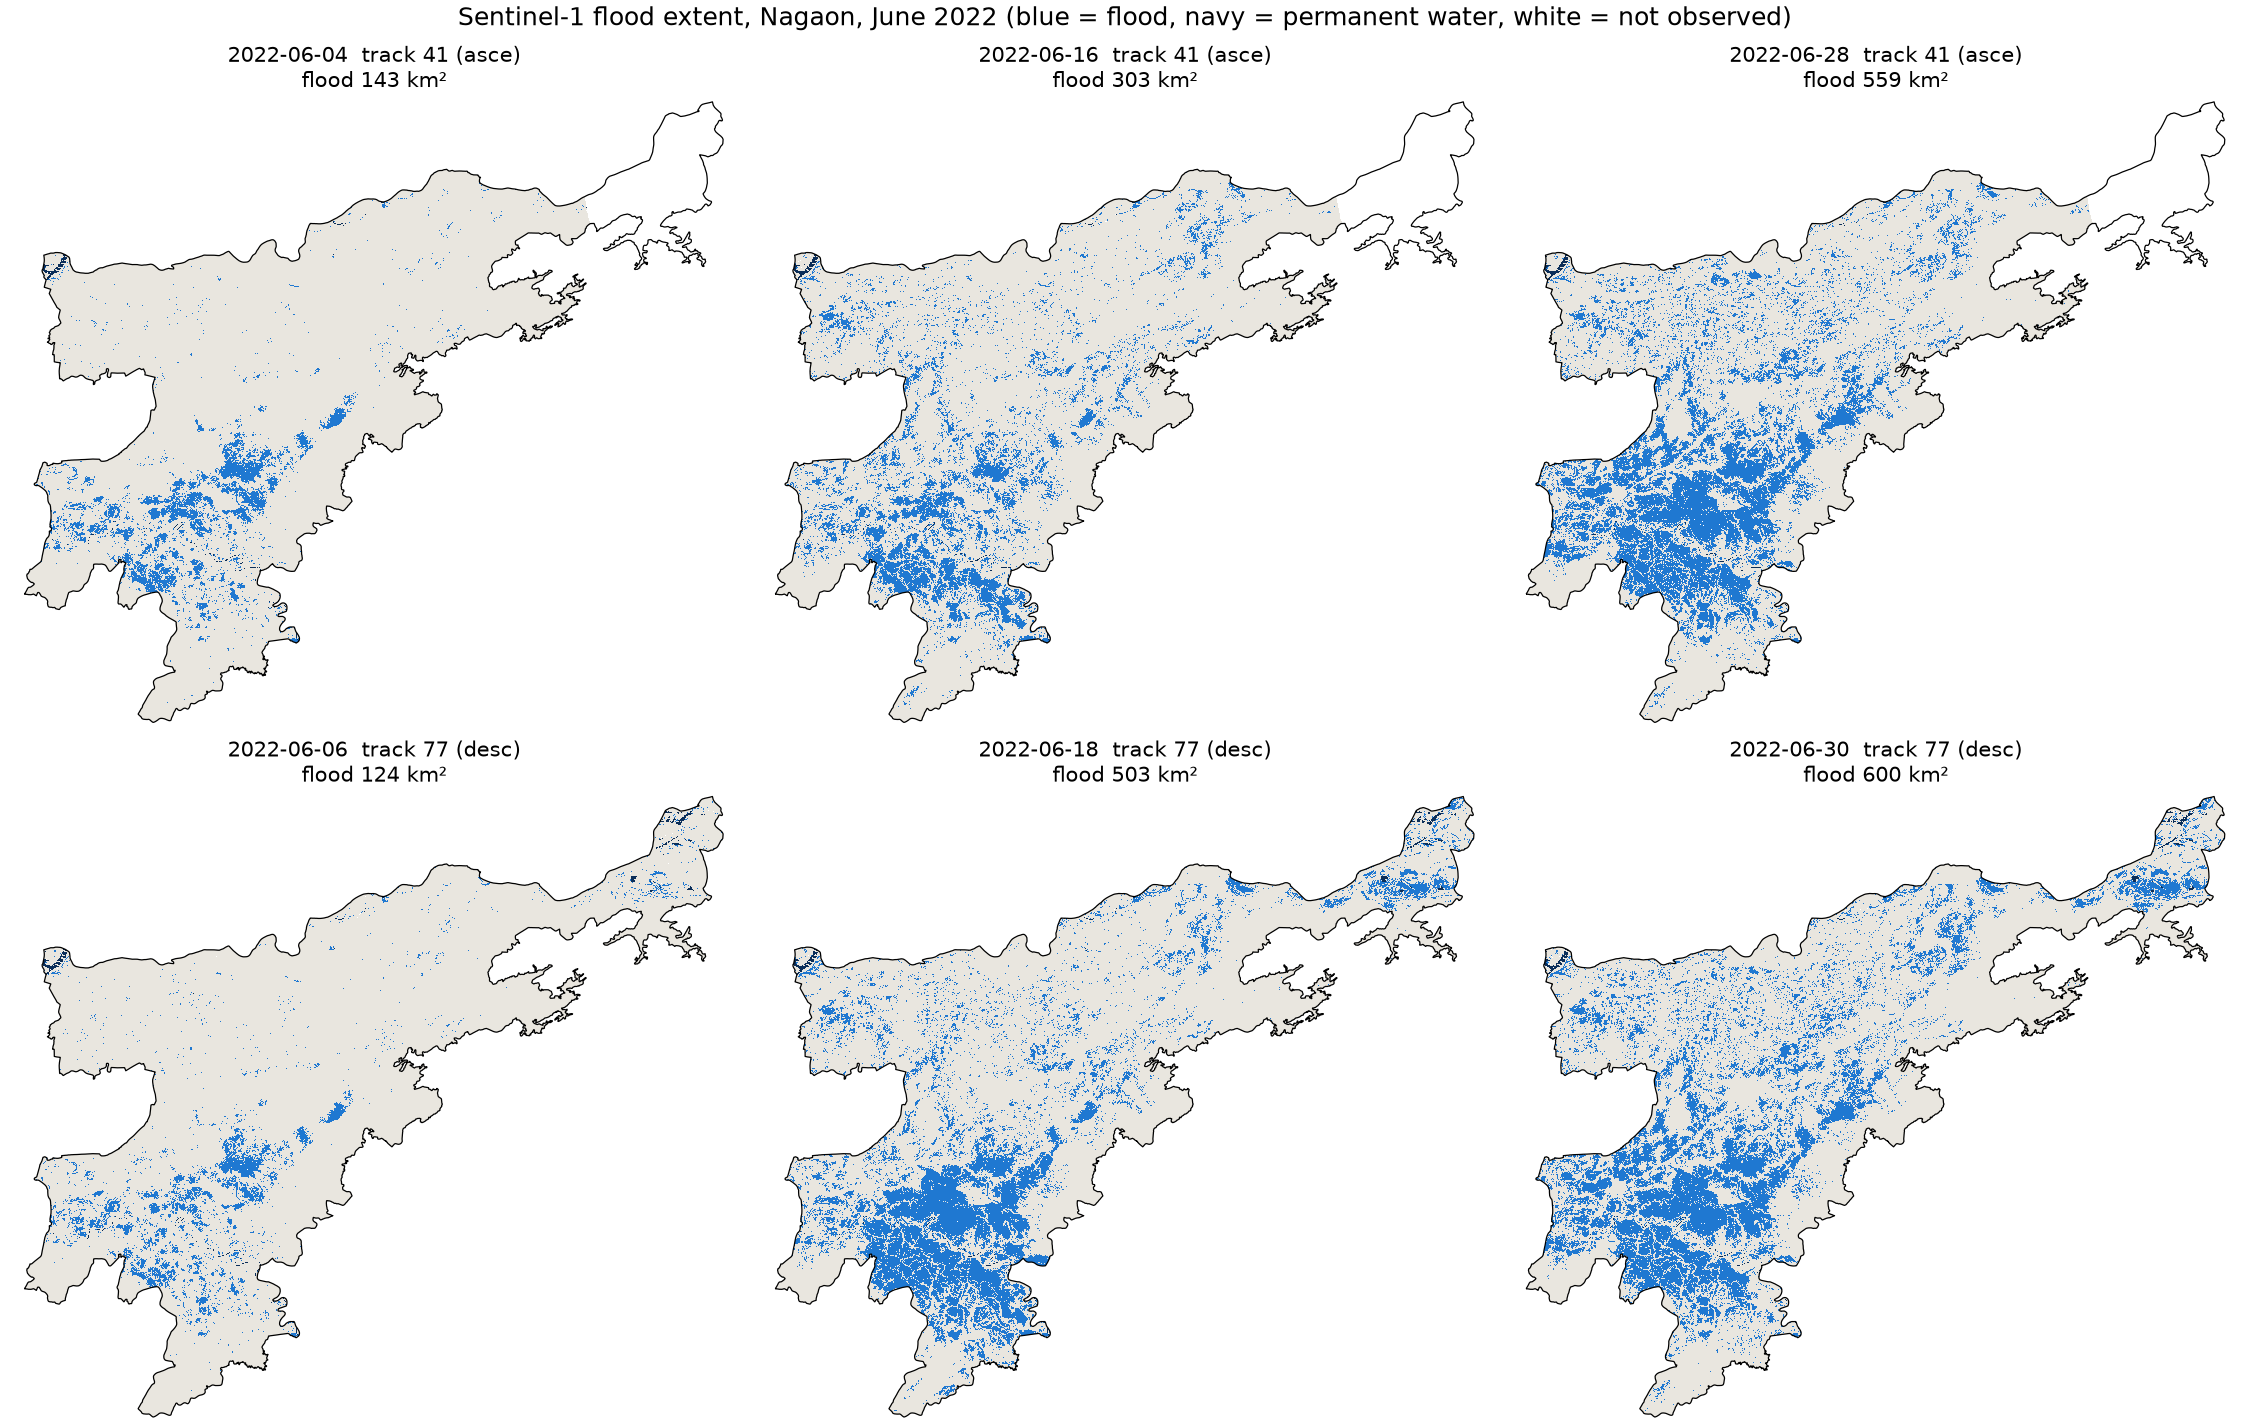
\includegraphics[width=\linewidth]{flood_maps_june2022.png}
\caption{Flood extent on the six Sentinel-1 dates (top: ascending track 41; bottom: descending track 77).
White areas were not observed by that track.}
\label{fig:six}
\end{figure}

\begin{figure}[H]
\centering
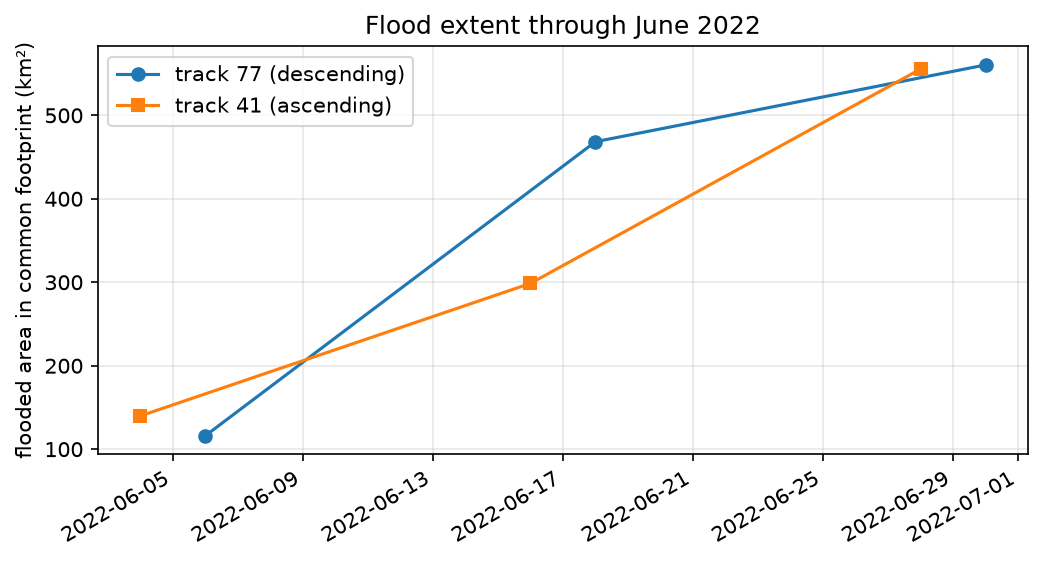
\includegraphics[width=0.72\linewidth]{flood_area_timeseries.png}
\caption{Flooded area in the footprint observed on all dates.}
\label{fig:ts}
\end{figure}

In total \SI{766}{\kmsq} (30\% of the district) was flooded on at least one date and \SI{405}{\kmsq} on three
or more (Figure~\ref{fig:freq}). The most persistent flooding lies in Raha, Kampur and the southern part of
Nagaon sub-district, in the Kopili--Kolong lowlands. The location of the worst flooding changed during the month
(Table~\ref{tab:subflood}): Kampur peaked on 18 June, whereas Raha and Nagaon reached their largest extent on
28--30 June.

\begin{figure}[H]
\centering
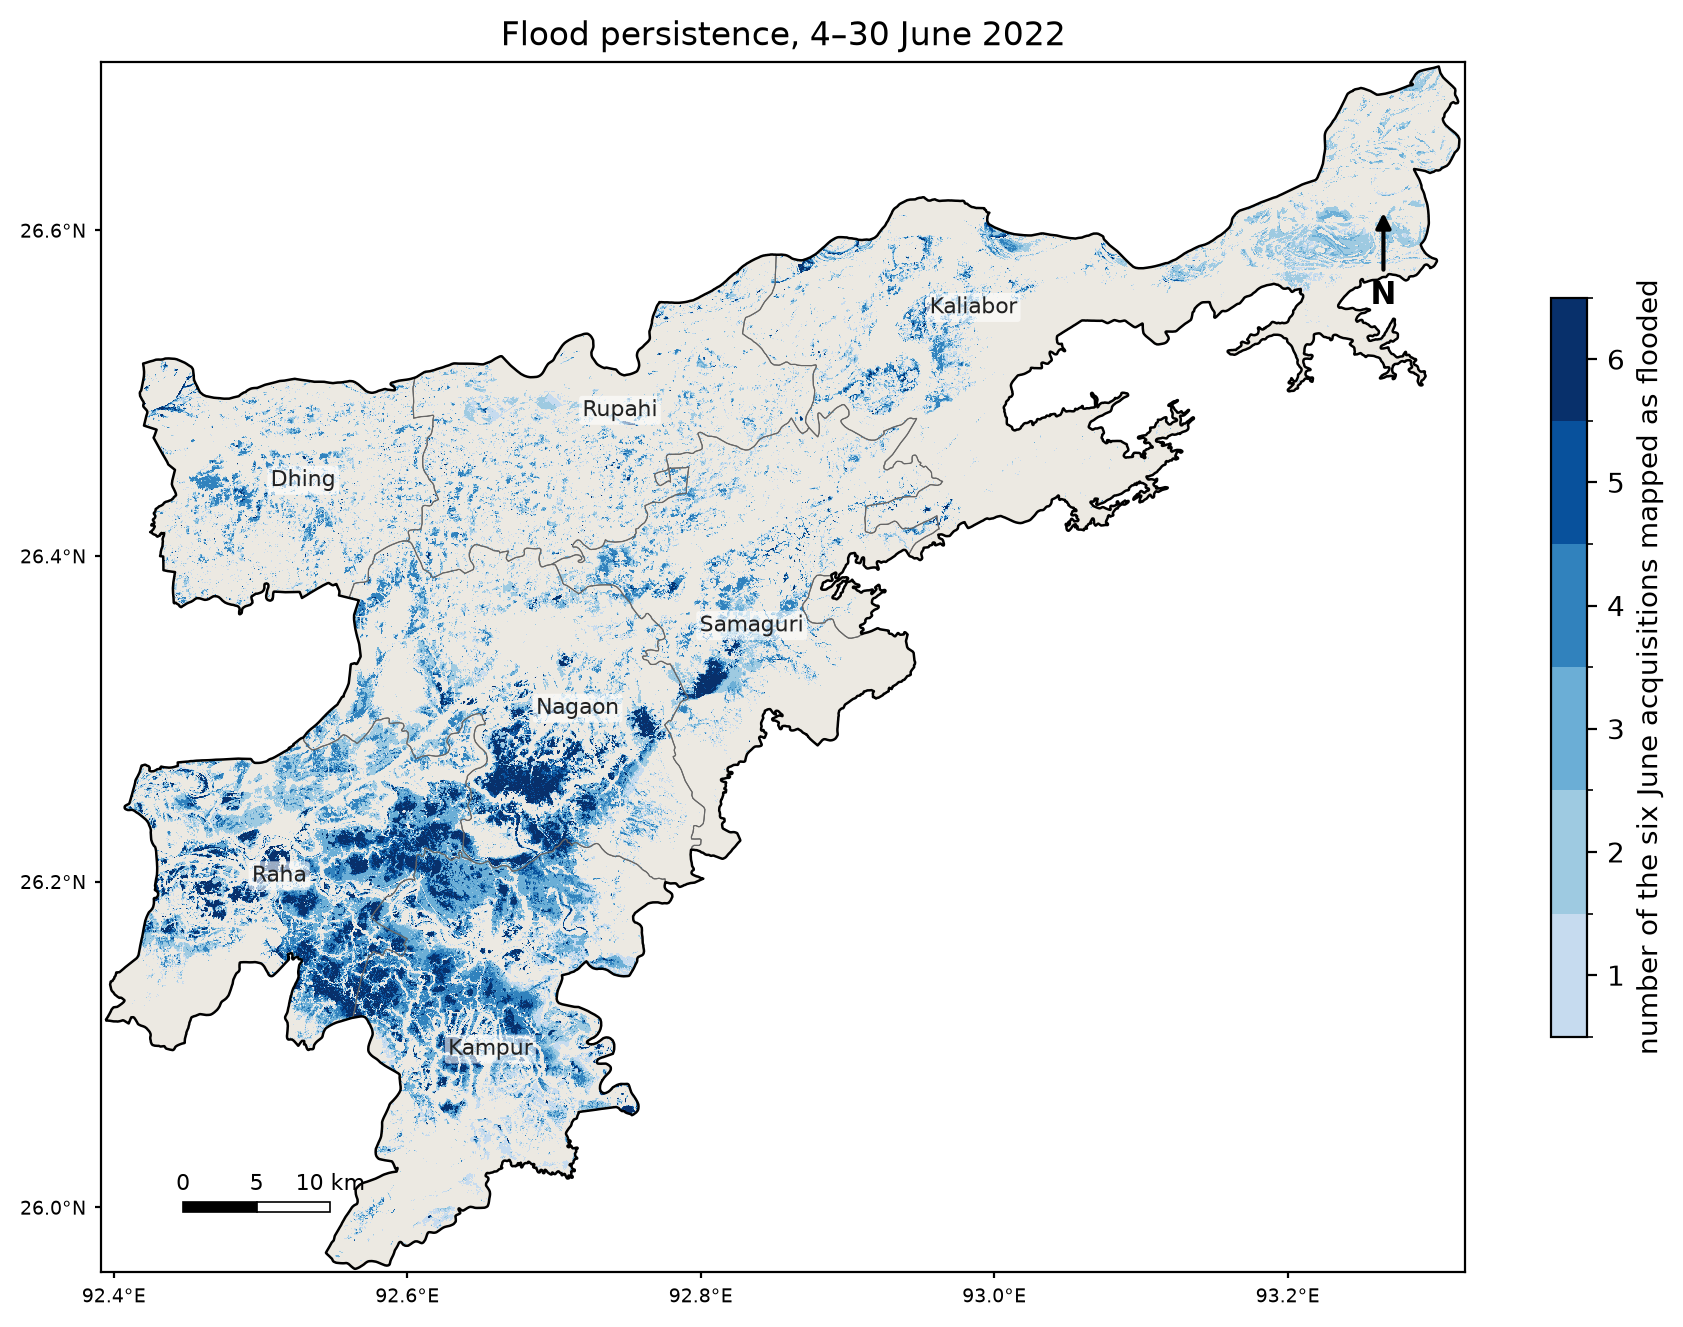
\includegraphics[width=0.82\linewidth]{map_flood_frequency.png}
\caption{Flood persistence: number of the six June acquisitions on which each pixel was mapped as flooded.
The eastern tip of Kaliabor was observed only by track 77 (three dates).}
\label{fig:freq}
\end{figure}

\begin{table}[H]
\centering\small
\caption{Flooded area (\kmsq) by sub-district and date.}
\label{tab:subflood}
\begin{tabular}{lrrrrrr}
\toprule
Sub-district & 4 Jun & 6 Jun & 16 Jun & 18 Jun & 28 Jun & 30 Jun\\
\midrule
Raha & 53.5 & 42.4 & 85.1 & 124.2 & \textbf{166.7} & 160.6\\
Kampur & 36.3 & 27.6 & 84.4 & \textbf{171.2} & 131.0 & 121.5\\
Nagaon & 40.6 & 34.5 & 54.3 & 74.7 & \textbf{116.5} & 114.9\\
Kaliabor & 2.6 & 9.5 & 20.4 & 57.5 & 27.2 & \textbf{74.9}\\
Samaguri & 6.6 & 5.7 & 26.3 & 32.2 & 52.1 & \textbf{56.4}\\
Rupahi & 1.6 & 2.2 & 11.4 & 18.4 & 35.0 & \textbf{36.9}\\
Dhing & 1.7 & 2.4 & 21.2 & 25.1 & 30.6 & \textbf{34.9}\\
\bottomrule
\end{tabular}\\[2pt]
{\footnotesize Kaliabor values from track 41 (4, 16, 28 June) exclude its unobserved eastern tip.}
\end{table}

\begin{figure}[H]
\centering
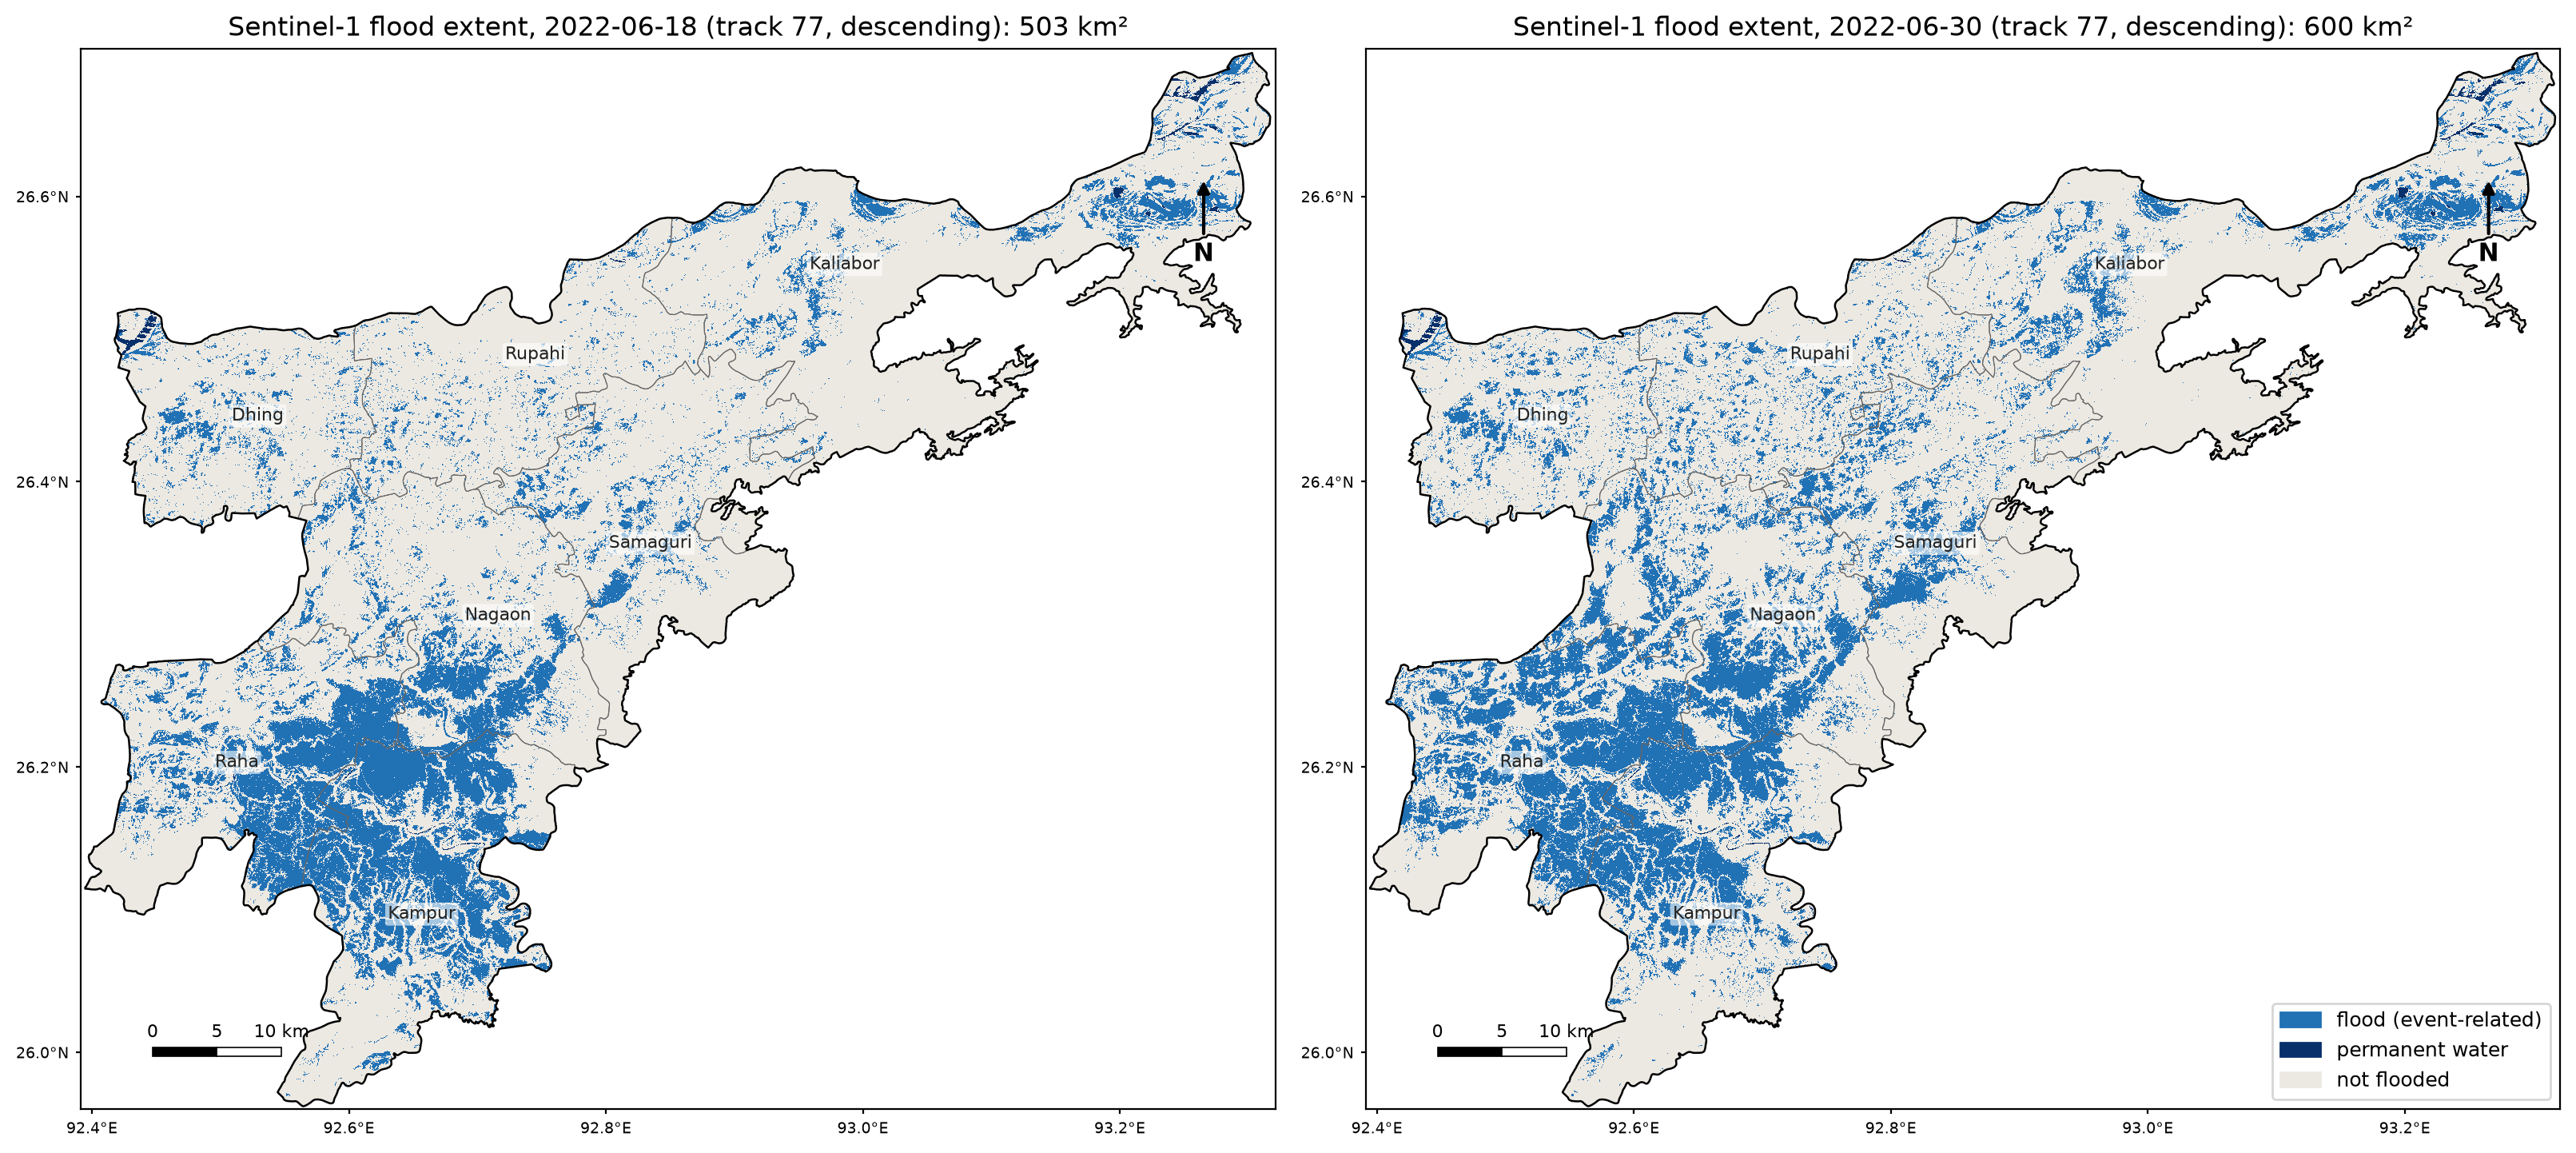
\includegraphics[width=\linewidth]{map_flood_extent.png}
\caption{Flood extent on 18 and 30 June 2022 (track 77, full district coverage).}
\label{fig:extent}
\end{figure}

\subsection{Settlement exposure (RQ ii)}
Table~\ref{tab:expo} summarises built-up land near flood water. On the peak date (30 June) \SI{4.6}{\kmsq}
of built-up land (7.2\%) lay within \SI{50}{m} of flooding; over the whole month the figure is
\SI{7.2}{\kmsq} (11.3\%), spread over \num{8806} of the district's \num{29799} built-up clusters. The choice of
distance matters: across all dates the exposed area ranges from \SI{2.6}{\kmsq} at \SI{30}{m} to
\SI{22.3}{\kmsq} at \SI{100}{m}.

\begin{table}[H]
\centering\small
\caption{Built-up land (WorldCover 2021) near mapped flood water (\kmsq).}
\label{tab:expo}
\begin{tabular}{lrrrr}
\toprule
Scenario & $\leq$ 30 m & $\leq$ 50 m (\% of built-up) & $\leq$ 100 m (\%) & Clusters $\leq$ 50 m\\
\midrule
4 June (t41) & 0.23 & 0.79 (1.3\%) & 3.03 (4.8\%) & \num{1011}\\
6 June (t77) & 0.32 & 1.00 (1.6\%) & 3.79 (5.9\%) & \num{1224}\\
16 June (t41) & 0.49 & 2.02 (3.2\%) & 8.63 (13.6\%) & \num{2921}\\
18 June (t77) & 1.21 & 3.60 (5.6\%) & 12.19 (19.1\%) & \num{4726}\\
28 June (t41) & 1.43 & 4.49 (7.1\%) & 16.02 (25.3\%) & \num{5826}\\
30 June (t77) & 1.35 & 4.61 (7.2\%) & 17.15 (26.8\%) & \num{6248}\\
\midrule
Any June date & 2.61 & 7.24 (11.3\%) & 22.30 (34.9\%) & \num{8806}\\
\bottomrule
\end{tabular}
\end{table}

\begin{table}[H]
\centering\small
\caption{Built-up land within 50 m of flooding on any June date, by sub-district.}
\label{tab:exposub}
\begin{tabular}{lrrr}
\toprule
Sub-district & Built-up (\kmsq) & Exposed (\kmsq) & Exposed (\%)\\
\midrule
Raha & 5.88 & 1.47 & \textbf{25.1}\\
Kampur & 3.56 & 0.81 & \textbf{22.7}\\
Dhing & 8.84 & 1.04 & 11.8\\
Rupahi & 9.35 & 1.10 & 11.7\\
Samaguri & 7.49 & 0.77 & 10.2\\
Nagaon & 21.26 & 1.64 & 7.7\\
Kaliabor & 7.57 & 0.42 & 5.5\\
\bottomrule
\end{tabular}
\end{table}

In absolute terms the largest exposed area is in Nagaon sub-district (\SI{1.64}{\kmsq}, which contains the town),
but the highest shares are in Raha and Kampur (Table~\ref{tab:exposub}, Figure~\ref{fig:expo}). The pixel-level view
near Raha shows that much of the exposed built-up class consists of roads and the houses lining them, running between
flooded fields: WorldCover's built-up class includes roads, so the exposure measure combines settlements and
transport infrastructure.

\begin{figure}[H]
\centering
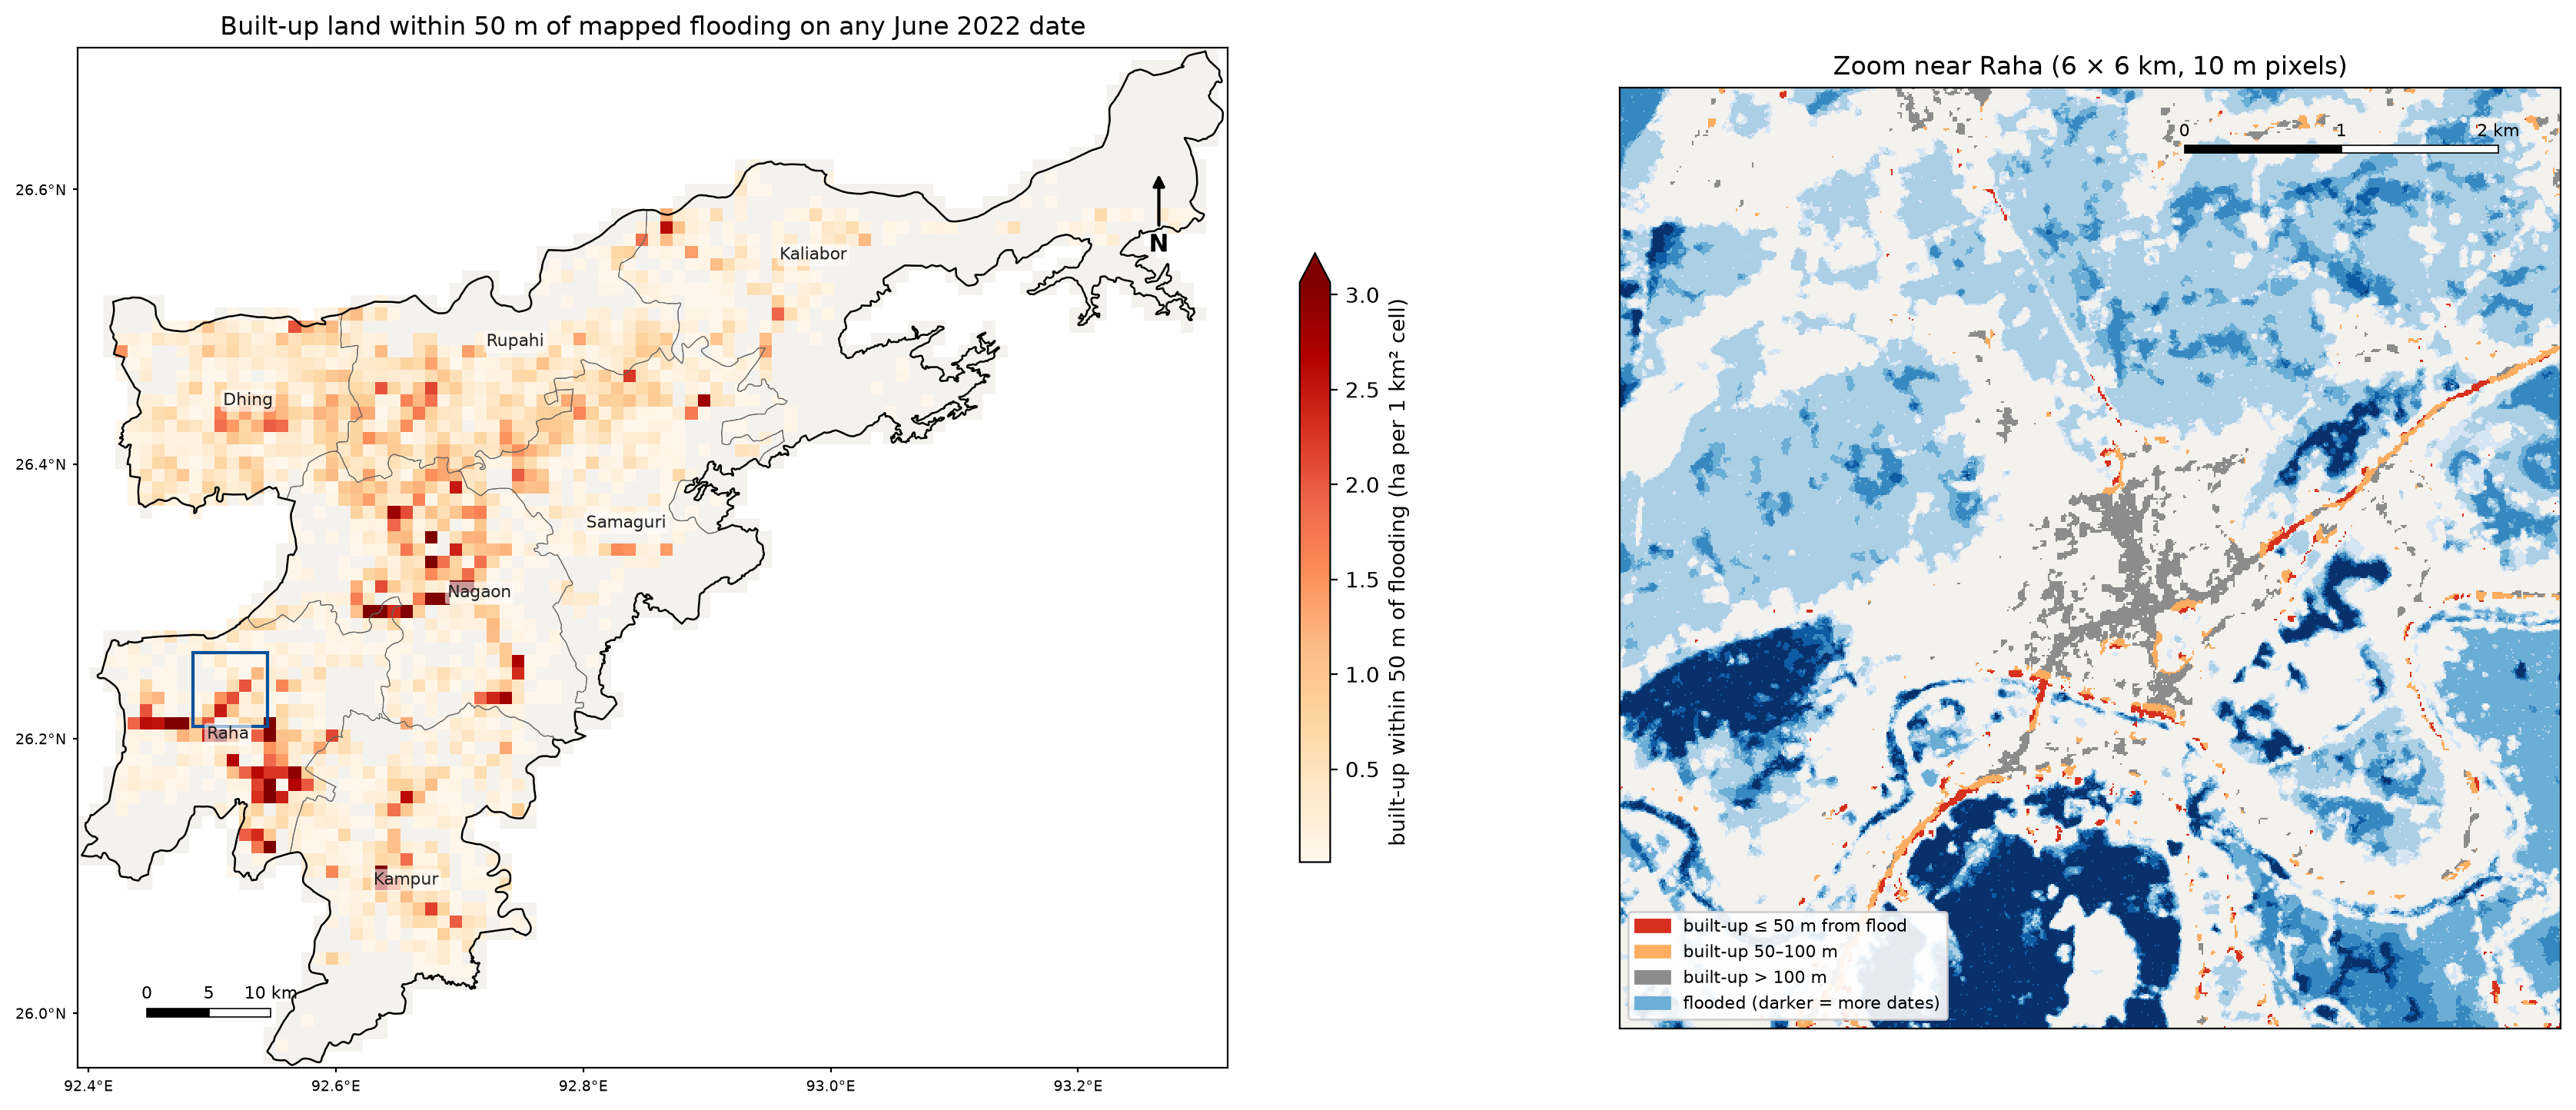
\includegraphics[width=\linewidth]{map_exposure.png}
\caption{Left: built-up land within 50 m of flooding on any June date, per 1 km cell. Right: 6 $\times$ 6 km
zoom near Raha at 10 m, showing built-up pixels by distance to flood water over flood persistence.}
\label{fig:expo}
\end{figure}

\subsection{Sensitivity to detection settings (RQ iii)}
Table~\ref{tab:sens} and Figure~\ref{fig:sens} summarise the one-at-a-time experiments. The VH-drop threshold has
by far the largest effect, followed by the absolute VH threshold. Over commonly used values of the two
(drop $-2$ to $-4$ dB, VH $-19$ to $-22$ dB; Figure~\ref{fig:joint}) the 18 June flooded area ranges from
\SI{423}{} to \SI{575}{\kmsq} ($-16\%$ to $+14\%$ of the default \SI{503}{\kmsq}). The permanent-water definition
matters because a large part of the floodplain has held water in some past months: excluding every pixel that JRC
has ever seen wet removes about \SI{90}{\kmsq} on 18 June. The terrain masks change the result by less than 1\%,
as expected in a flat floodplain. VV detects about 10\% less flooding than VH. Exposure follows flood area but is
proportionally more sensitive, especially to the minimum patch size, because small flood patches next to houses
are the first to be removed.

\begin{table}[H]
\centering\small
\caption{Sensitivity of flooded area to each setting (one-at-a-time, 16, 18 and 30 June).}
\label{tab:sens}
\begin{tabularx}{\linewidth}{>{\raggedright}p{3.6cm}>{\raggedright}p{3.0cm}>{\raggedright}p{2.6cm}X}
\toprule
Setting & Range tested & Area range (\% of default) & Note\\
\midrule
VH-drop threshold & $-1$ to $-6$ dB & 43--73\% & 18 Jun: 358--574 \kmsq\\
Absolute VH threshold & $-17$ to $-24$ dB & 32--37\% & 18 Jun: 373--534 \kmsq\\
Permanent-water definition & JRC $\geq$ 1--12 months, none & 16--19\% & strictest removes $\sim$90 \kmsq{} on 18 Jun\\
Minimum patch & 1--100 px & 6--11\% & exposure 2.5--4.5 \kmsq{} on 18 Jun\\
Polarisation & VH, VV & 7--10\% & VV Otsu threshold $-13.1$ dB\\
HAND, slope & 5 m--off, \ang{2}--off & $<$ 1\% & flat floodplain\\
\bottomrule
\end{tabularx}
\end{table}

\begin{figure}[H]
\centering
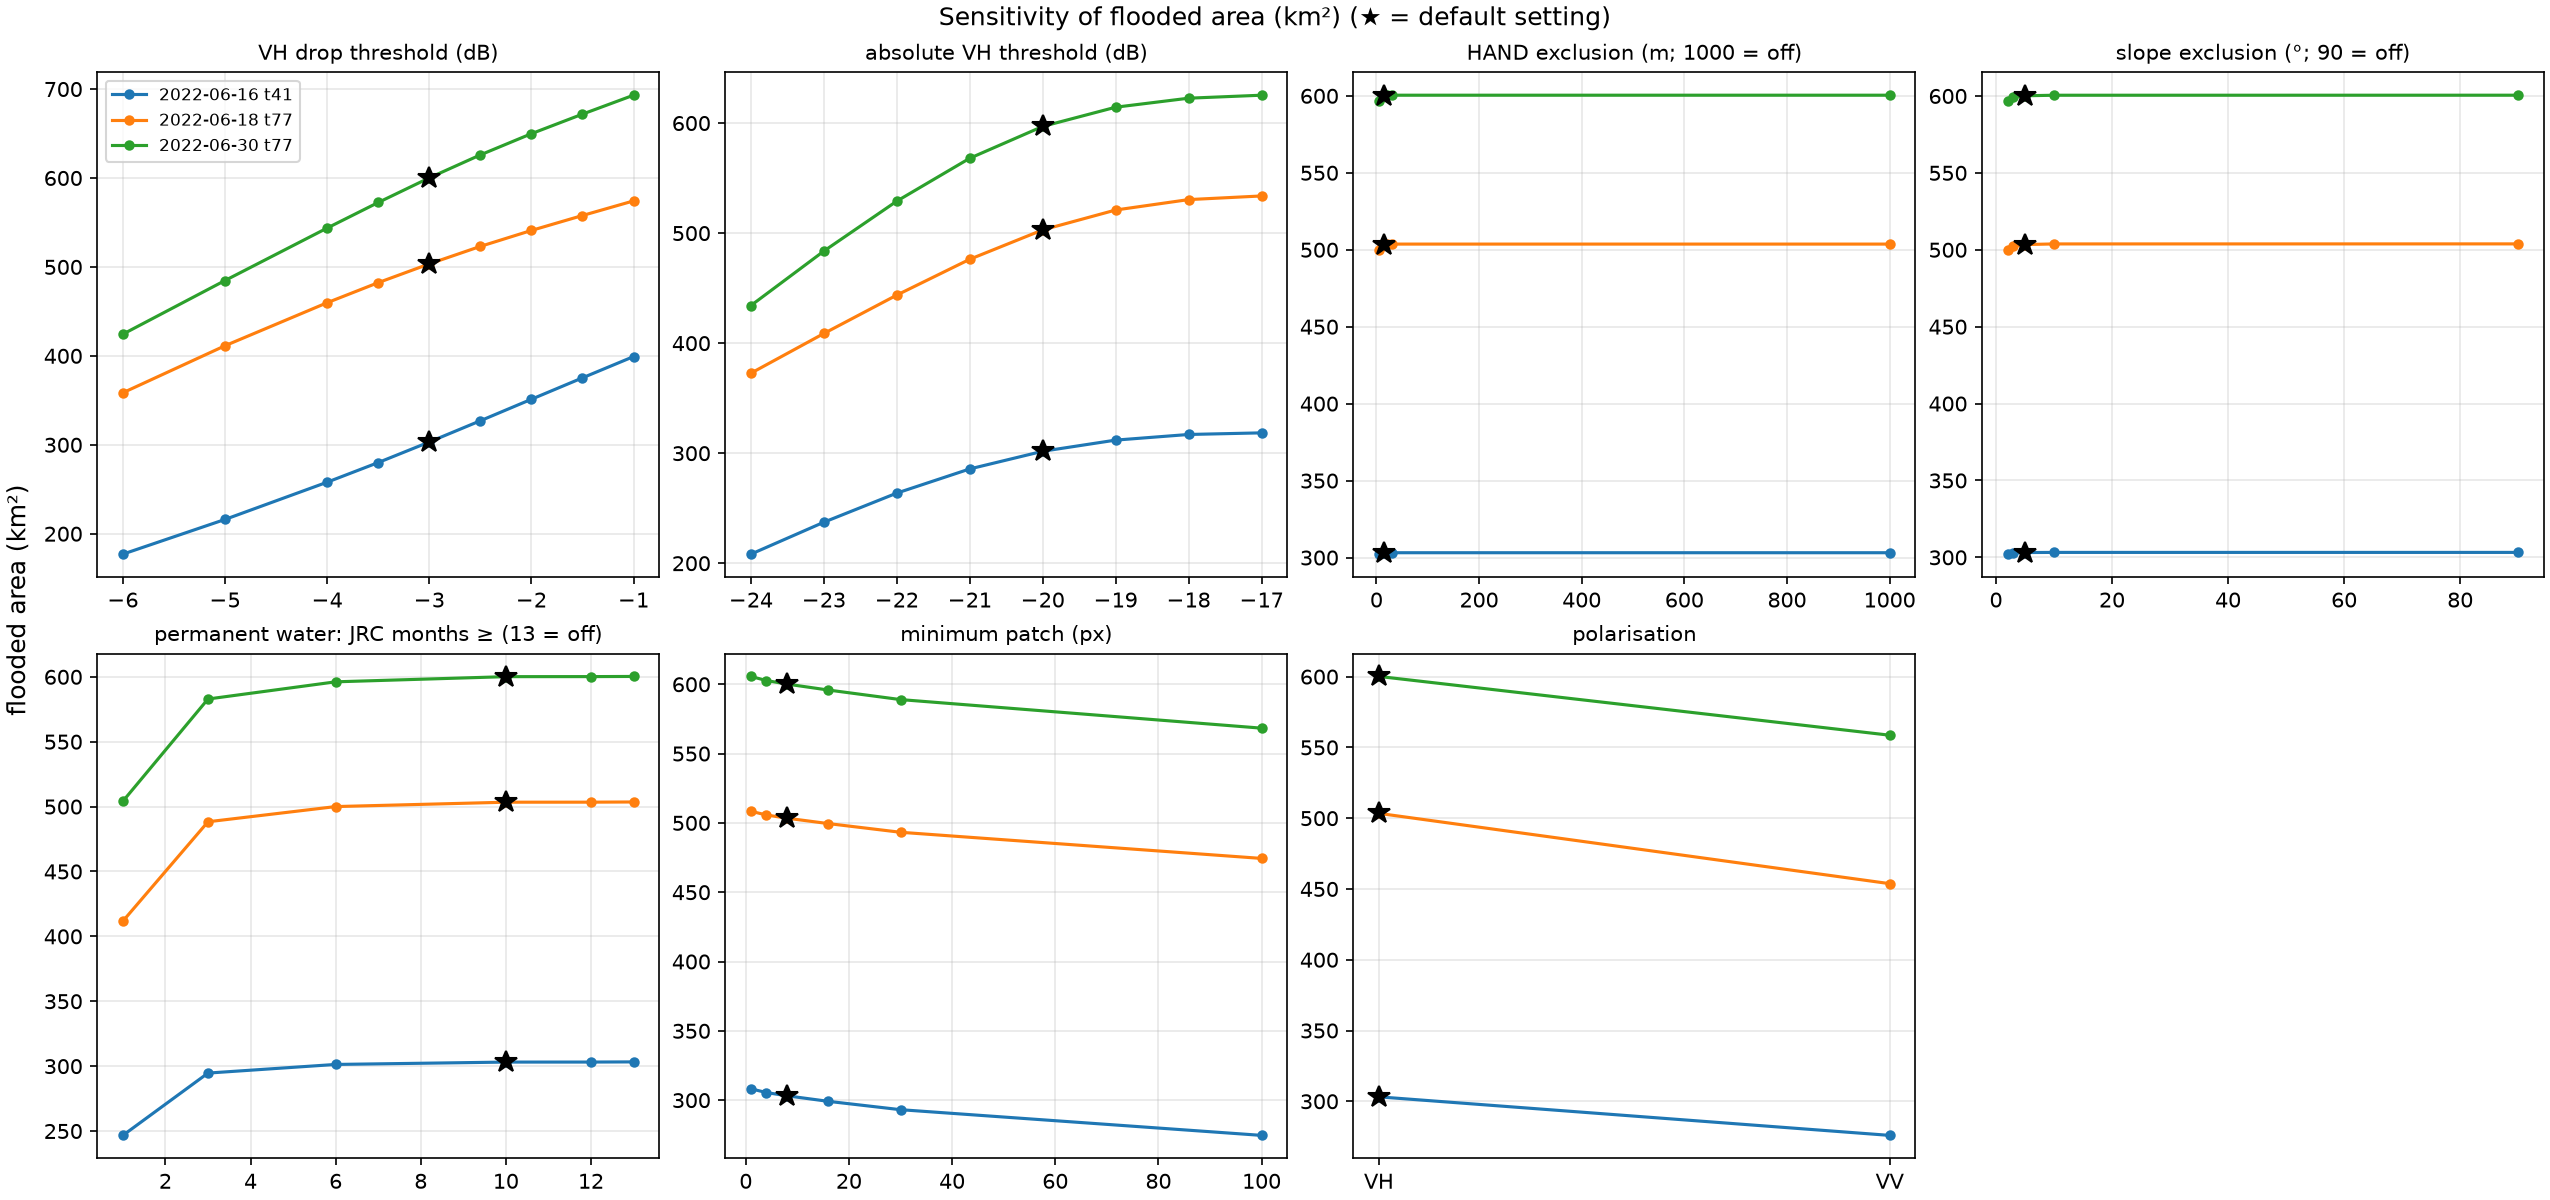
\includegraphics[width=\linewidth]{sensitivity_flood_area.png}
\caption{Flooded area as each setting is varied (stars mark the defaults).}
\label{fig:sens}
\end{figure}

\begin{figure}[H]
\centering
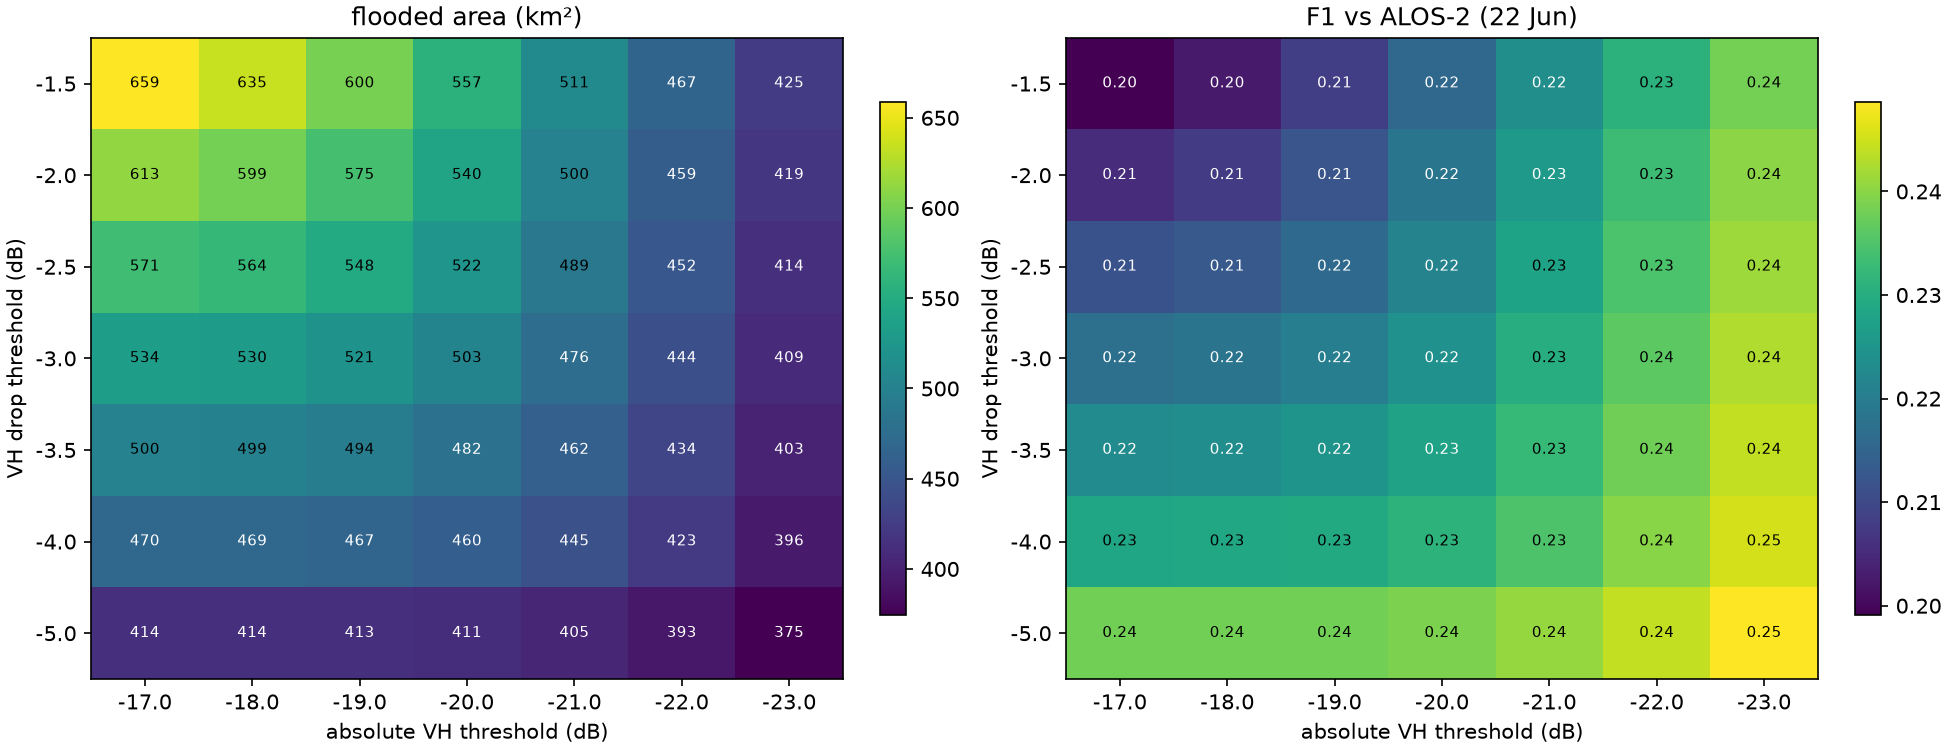
\includegraphics[width=\linewidth]{sensitivity_joint_18jun.png}
\caption{Joint variation of the two main thresholds on 18 June: flooded area and F1 agreement with the ALOS-2 map.}
\label{fig:joint}
\end{figure}

Agreement with the reference maps changes little across settings (F1 0.41--0.48 against MBRSC and 0.16--0.25
against ALOS-2), so the references alone cannot identify a single best threshold; stricter thresholds raise F1
against ALOS-2 slightly because that product is conservative.

\subsection{Agreement with reference maps and published estimates}
\begin{table}[H]
\centering\small
\caption{Pixel agreement with reference flood maps (all observed pixels in the district).}
\label{tab:val}
\setlength{\tabcolsep}{4pt}
\begin{tabular}{llrrrrrrr}
\toprule
Reference & Our map & Ref. (\kmsq) & Ours (\kmsq) & Precision & Recall & F1 & OA & $\kappa$\\
\midrule
MBRSC (S1, 16 Jun) & 16 Jun, t41 & 128.1 & 303.1 & 0.33 & 0.78 & 0.46 & 0.90 & 0.42\\
ALOS-2 (22 Jun) & 18 Jun, t77 & 143.7 & 503.4 & 0.14 & 0.51 & 0.22 & 0.81 & 0.15\\
ALOS-2 (22 Jun) & 28 Jun, t41 & 135.0 & 559.0 & 0.12 & 0.50 & 0.20 & 0.77 & 0.12\\
\bottomrule
\end{tabular}
\end{table}

Against the MBRSC map derived from the same Sentinel-1 scene, our map captures 78\% of the reference flooding,
but maps more than twice the area (Table~\ref{tab:val}). Against the independent ALOS-2 map, half of the reference
flooding is captured. Agreement is better at coarser scales (Figure~\ref{fig:cells}): the correlation of flood
fractions rises from 0.57 at 100 m to 0.61 at 1 km for MBRSC and from 0.28 to 0.57 for ALOS-2. Sub-district
totals are ranked consistently (Spearman $\rho$ = 0.82 against MBRSC and 0.86 against ALOS-2 for 18 June).

\begin{figure}[H]
\centering
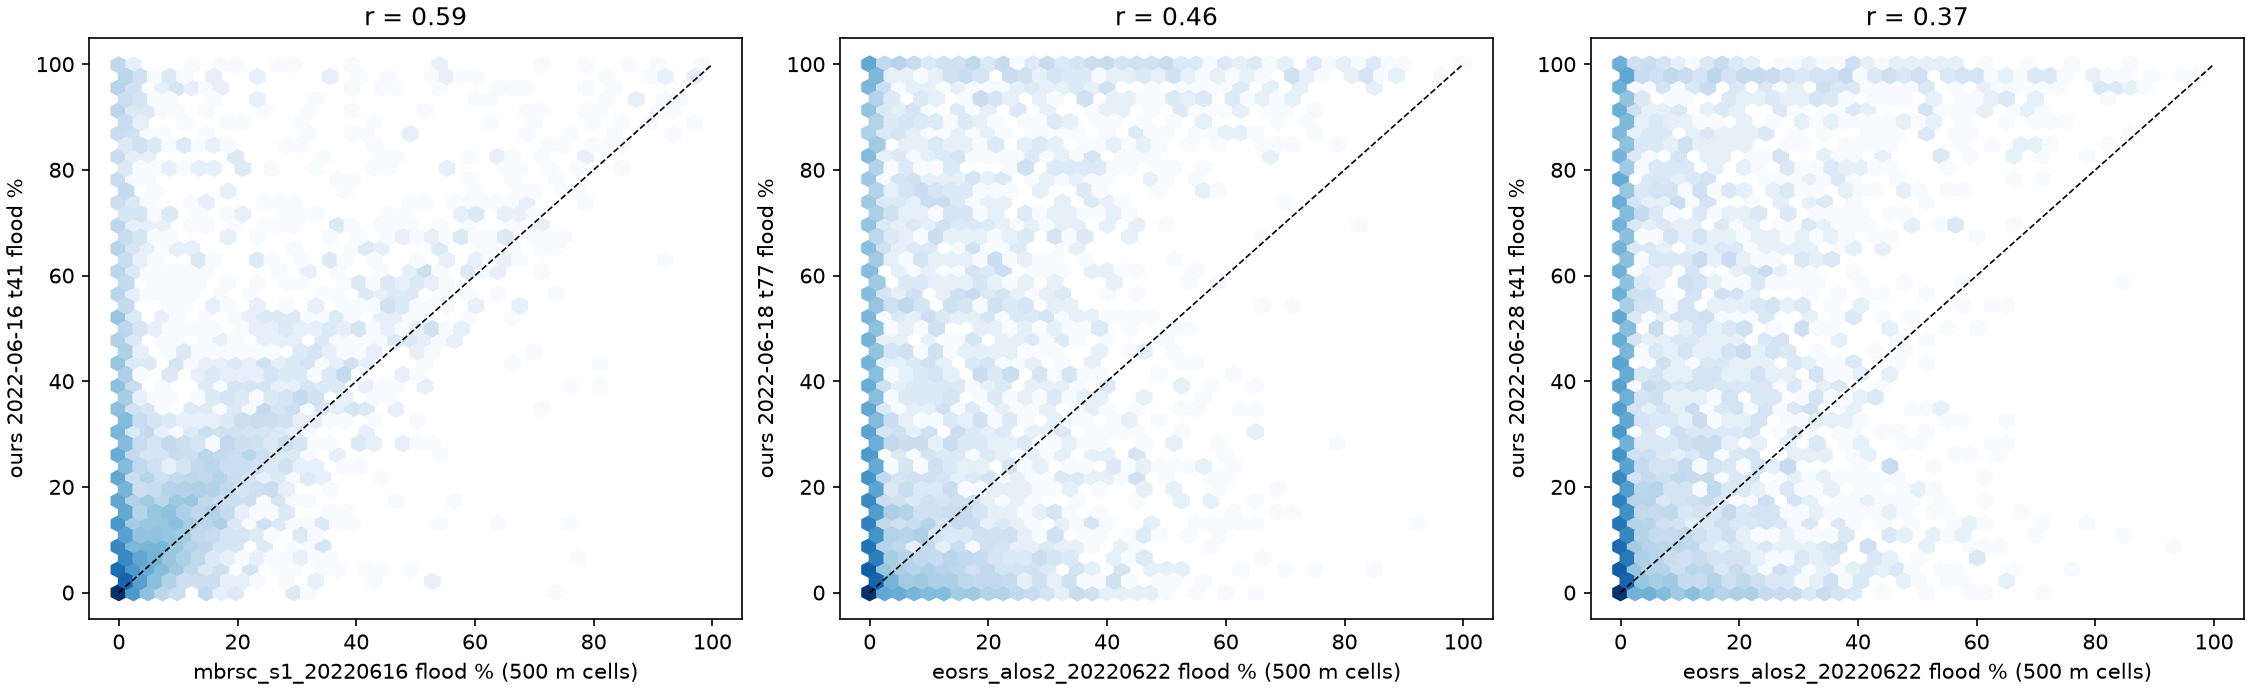
\includegraphics[width=\linewidth]{validation_cell_scatter.png}
\caption{Flood fraction in 500 m cells: our maps versus the reference maps.}
\label{fig:cells}
\end{figure}

The disagreements are systematic. Of the \SI{431}{\kmsq} mapped only by us on 18 June, \SI{378}{\kmsq} is cropland
and 46\% lies where JRC has recorded water before, consistent with waterlogged or flooded paddy and seasonal wetlands.
Of the \SI{71}{\kmsq} mapped only in the ALOS-2 product, \SI{36}{\kmsq} is tree cover: L-band radar penetrates the
canopy and detects water beneath it, whereas C-band Sentinel-1 does not.

\begin{table}[H]
\centering\small
\caption{Flooded area in Nagaon from published sources and this study.}
\label{tab:pub}
\begin{tabular}{lrr}
\toprule
Source & 18 June 2022 (\kmsq) & 30 June 2022 (\kmsq)\\
\midrule
NRSC reference, as cited by \cite{irukumati} & 413.3 & 597.3$^{*}$\\
Random Forest, VV / VH / VV+VH \cite{irukumati} & 395.6 / 383.2 / 400.3 & 565.3 / 583.2 / 592.1\\
K-means, VV / VH / VV+VH \cite{irukumati} & 413.3 / 389.2 / 401.8 & 613.2 / 592.6 / 551.9\\
\textbf{This study} (VH change detection) & \textbf{503.4} & \textbf{600.1}\\
\bottomrule
\end{tabular}\\[2pt]
{\footnotesize $^{*}$ Read from a table column that is split across the PDF layout of the source.}
\end{table}

The 30 June area agrees with the NRSC figure to within 1\% and lies inside the spread of the classifiers tested by
\cite{irukumati} (Table~\ref{tab:pub}). On 18 June our estimate is about 22\% higher than NRSC; this difference is
within the threshold-sensitivity range (for example, a $-22$ dB VH threshold gives \SI{444}{\kmsq}). The rapid-mapping
proxy products (\SIrange{128}{144}{\kmsq}) are much smaller than both NRSC's figures and ours, which suggests that they
were deliberately conservative.

Finally, 15\% of the 18 May flood area was flooded again on 4--6 June, rising to 50--57\% by 18--30 June. Using a
January--April baseline therefore avoids treating residual May water as dry ground.

% ------------------------------------------------------------------ 6
\section{Discussion}
\paragraph{Temporal pattern.} Two independent orbit tracks give a consistent picture of a flood that grew rapidly in
mid-June and stayed extensive until the end of the month. Using both tracks doubled the number of observations to six,
which was valuable after the loss of Sentinel-1B.

\paragraph{What the maps include and miss.} The change-detection maps are more inclusive than the rapid-mapping
products. Commission is concentrated in cropland and historically wet land, where flooded paddy fields, waterlogged
fields after heavy rain and seasonal wetlands all darken in the same way as flood water; a dry-season baseline cannot
separate them, and late June is the start of the sali rice transplanting season. Omission is concentrated under trees
and among buildings, where C-band backscatter does not drop. Rural settlements in Nagaon are often villages under
homestead trees, which WorldCover classifies as tree cover rather than built-up, so both the flood maps and the
exposure estimate are likely to understate flooding in and around villages.

\paragraph{Exposure measure.} Because SAR cannot see water among buildings, a proximity measure is necessary, but its
value depends strongly on the chosen distance (a factor of about eight between 30 and 100 m). The \SI{50}{m} figure
should be read as an indicator of where settlements and roads were close to flood water, not as a count of flooded
houses or affected people.

\paragraph{Threshold choice.} Results are robust to terrain settings but sensitive to the two backscatter thresholds,
giving an uncertainty of roughly $\pm$15\% in flooded area for reasonable choices. Reporting this range is more honest
than reporting a single number.

\subsection*{Limitations}
\begin{itemize}
\item C-band SAR misses flooding beneath vegetation and among buildings; exposure is a proximity indicator and a likely lower bound for settlements under tree cover.
\item Flooded paddy and seasonal wetlands may be counted as flood; the dry-season baseline cannot distinguish them.
\item Track 41 does not observe the eastern tip of Kaliabor; cross-track comparisons use the common footprint.
\item The reference products are rapid-mapping outputs with unknown accuracy and differ in date (ALOS-2 on 22 June lies between our 18 and 28 June scenes); NRSC/ASDMA GIS layers were not publicly available.
\item WorldCover built-up includes roads; built-up clusters are not villages; 2011-census sub-districts are used as reporting units and do not exactly match current revenue circles.
\end{itemize}

% ------------------------------------------------------------------ 7
\section{Conclusions}
\begin{enumerate}[label=(\roman*)]
\item Inundation in Nagaon increased from about \SI{125}{}--\SI{145}{\kmsq} in early June 2022 to \SI{503}{\kmsq} on
18 June and \SI{600}{\kmsq} on 30 June; \SI{766}{\kmsq} (30\% of the district) was flooded on at least one date, with the
most persistent flooding in Raha, Kampur and southern Nagaon.
\item \SI{7.2}{\kmsq} of built-up land (11\%) lay within \SI{50}{m} of flood water at some point in June. Raha and Kampur
had the highest proportion of built-up land exposed (about a quarter), while Nagaon sub-district had the largest
absolute area.
\item Flood extent is most sensitive to the backscatter-drop and absolute VH thresholds ($\pm$15\% for common choices),
moderately sensitive to the permanent-water definition, and insensitive to terrain masks. Exposure is more sensitive than
flood extent, particularly to the proximity distance and minimum patch size.
\end{enumerate}
The method reproduces the NRSC flood area for 30 June and gives consistent sub-district rankings against independent
products. Combining Sentinel-1 with L-band SAR (for flooding under vegetation) and with a building footprint or population
dataset (for exposure) would be the most useful extensions.

% ------------------------------------------------------------------ references
\begin{thebibliography}{9}\small
\bibitem{twele} Twele, A., Cao, W., Plank, S. and Martinis, S. (2016). Sentinel-1-based flood mapping: a fully automated
processing chain. \emph{International Journal of Remote Sensing}, 37(13), 2990--3004. doi:10.1080/01431161.2016.1192304
\bibitem{irukumati} Irukumati, S., Vittal, A. R. and Gurunarayan, S. L. (2025). Comparative analysis of classification
techniques for flood mapping using Sentinel 1 SAR data. \emph{Environmental Earth Sciences}, 84, 398.
doi:10.1007/s12665-025-12381-3
\bibitem{donchyts} Donchyts, G., Schellekens, J., Winsemius, H., Eisemann, E. and van de Giesen, N. (2016). A 30 m
resolution surface water mask including estimation of positional and thematic differences using Landsat 8, SRTM and
OpenStreetMap: a case study in the Murray--Darling Basin, Australia. \emph{Remote Sensing}, 8(5), 386.
\bibitem{lee} Lee, J.-S. (1980). Digital image enhancement and noise filtering by use of local statistics. \emph{IEEE
Transactions on Pattern Analysis and Machine Intelligence}, 2(2), 165--168.
\bibitem{pekel} Pekel, J.-F., Cottam, A., Gorelick, N. and Belward, A. S. (2016). High-resolution mapping of global surface
water and its long-term changes. \emph{Nature}, 540, 418--422.
\bibitem{merit} Yamazaki, D., Ikeshima, D., Sosa, J., Bates, P. D., Allen, G. H. and Pavelsky, T. M. (2019). MERIT Hydro: a
high-resolution global hydrography map based on latest topography dataset. \emph{Water Resources Research}, 55, 5053--5073.
\bibitem{worldcover} Zanaga, D. et al. (2022). ESA WorldCover 10 m 2021 v200. doi:10.5281/zenodo.7254221
\bibitem{gee} Gorelick, N., Hancher, M., Dixon, M., Ilyushchenko, S., Thau, D. and Moore, R. (2017). Google Earth Engine:
planetary-scale geospatial analysis for everyone. \emph{Remote Sensing of Environment}, 202, 18--27.
\bibitem{sa} Sentinel Asia (2022). Flood in India, 15 June 2022 and 15 May 2022 event pages: EOS-RS Flood Proxy Maps and
MBRSC flood maps. \url{https://sentinel-asia.org/EO/2022/article20220615IN.html}
\end{thebibliography}

% ------------------------------------------------------------------ appendix
\appendix
\section{Reproducibility}
All processing is scripted in the project repository. Notebooks 01--06 cover the scene inventory, flood detection,
exposure, sensitivity, validation and maps; \texttt{src/} holds the shared code (Earth Engine preprocessing in
\texttt{floodmap.py}, local classification and metrics in \texttt{classify.py}). Sentinel-1 stacks were downloaded from
Earth Engine on a fixed 10 m UTM 46N grid; classification, statistics and figures then run locally. Output GeoTIFFs
(flood maps, flood frequency, exposure classes) are provided with QGIS style files.

\end{document}
